\documentclass[12pt]{mwart}

\usepackage{polski}
\usepackage[utf8]{inputenc}
\usepackage{mathtools,amsthm,amssymb,icomma,upgreek,xfrac,graphics,scrextend,float,tabularx,hyperref,multicol,array,caption,enumitem}
\usepackage[table,xcdraw]{xcolor}

\mathtoolsset{mathic}
\raggedbottom
\graphicspath{ {./images/} }
\renewcommand{\refname}{Źródła}
\captionsetup{justification=raggedright,singlelinecheck=true}


\begin{document}
	
	\begin{center}
		{\Large\textbf{Statystyka stosowana}}
	\end{center}
	\begin{center}
		Raport 2
	\end{center}
	
	\noindent Temat: \ \textbf{Testowanie hipotez statystycznych}\\
	Imię i Nazwisko prowadzącego kurs: \ \textbf{Mgr Katarzyna Maraj-Zygmąt}	\newline\newline
	
	
	\noindent\begin{tabularx}{\textwidth}{|X |X|}
		\hline
		\begin{center}
			Imię i Nazwisko,\\ nr indeksu
		\end{center} &  \begin{center}
			Szymon Malec, 262276\\
			Filip Oszczepaliński, 262292
		\end{center}\\\hline
		Wydział: & Wydział matematyki, W13 \\\hline
		Dzień i godzina zajęć: & Wtorek,\vphantom{ $11^{1^{5}}$} $7^{30}$\\\hline
		Kod grupy ćwiczeniowej: & T00-64c \\\hline
		Data oddania raportu: & 21.06.2022 \\\hline
		\textbf{Ocena końcowa} &\\\hline
	\end{tabularx}\newline\newline
	
	\noindent\textbf{Adnotacje i uwagi:}
	
	\newpage
	
	
	\section{Wstęp}
	
	\noindent Celem raportu jest rozwiązanie trzech zadań dostępnych na stronie \cite{zadania}. Zadania te dotyczą dwóch zbiorów danych pochodzących z rozkładów normalnych. Naszym zadaniem jest przeprowadzenie testów statystycznych w celu zweryfikowania prawdziwości podanych w zadaniach hipotez oraz wyznaczenie metodą Monte Carlo prawdopodobieństwa popełnienia błędów I i II rodzaju.
	
	
	
	\section{Potrzebne definicje}
	\subsection{Obszar krytyczny}
	\noindent Obszarem krytycznym nazywamy taki przedział, do którego należenie statystyki testowej prowadzi do odrzucenia hipotezy zerowej i przyjęcia hipotezy alternatywnej.
	\subsection{P-wartość}
	\noindent P-wartością prowadzonego testu nazywamy najmniejszy poziom istotności $\alpha$, przy którym zaobserwowana wartość statystyki testowej prowadzi do odrzucenia hipotezy zerowej.
	\subsection{Błąd I rodzaju}
	\noindent Odrzucenie hipotezy zerowej, gdy jest ona prawdziwa, nazywamy błędem I rodzaju.
	\subsection{Błąd II rodzaju}
	\noindent Przy zadanej alternatywnej wartości parametru $\theta$ będącego przedmiotem testowania, błędem II rodzaju nazywamy przyjęcie hipotezy zerowej, gdy jest ona fałszywa.
	\subsection{Moc testu}
	\noindent Dla danej alternatywnej wartości $\theta$, prawdopodobieństwa odrzucenia fałszywej hipotezy zerowej i przyjęcia prawdziwej hipotezy alternatywnej nazywamy mocą testu dla tej wartości.
	
	
	
	\section{Testowanie hipotez dotyczących wartości średniej}
	
	\noindent Zadanie 1 polega na zbadaniu próby $X_1, \dots, X_n$ z populacji generalnej o rozkładzie normalnym $\mathcal{N}(\mu\ , 0.2)$. Dane można odnaleźć na stronie \cite{dane1}. Długość próby wynosi $n = 1000$. Oznaczmy $\sigma^2 = 0,2$ oraz $\mu_0 = 1,5$. Naszym zadaniem jest zweryfikowanie hipotezy zerowej
	$$ \mathrm{H_0}: \mu = \mu_0 = 1,5 $$
	na poziomie istotności $\alpha = 0,05$. W tym celu konstruujemy statystykę
	$$ Z = \frac{\bar{X}-\mu_0}{\frac{\sigma}{\sqrt{n}}}, $$
	gdzie
	$$ \bar{X} = \frac{1}{n} \sum_{i=1}^n X_i $$
	jest nieobciążonym estymatorem parametru $\mu$. Jeśli hipoteza zerowa jest prawdziwa, to
	$$ Z \sim \mathcal{N}(0,1). $$
	Jeśli $\mathrm{H_0}$ jest fałszywa, statystyka $Z$ będzie miała tendencję do przyjmowania dużych lub małych wartości. Dla naszych danych wartość statystyki wynosi {\boldmath$-3.149$}. Hipotezę zerową będziemy testować naprzeciw trzem hipotezom alternatywnym.
	\begin{enumerate}[label=(\textbf{\alph*})]
		
		\item {\boldmath $\mathrm{H_1}: \mu \neq \mu_0$}\\
		Definiujemy obszar krytyczny jako przedział
		$$ C = \left( -\infty \ ; \ -z_{1-\frac{\alpha}{2}} \right] \cup \left[ z_{1-\frac{\alpha}{2}} \ ; \ \infty \right), $$
		gdzie  $z_{1-\frac{\alpha}{2}}$  jest kwantylem rzędu $1 - \frac{\alpha}{2}$ rozkładu  $\mathcal{N}(0,1)$ . Jeśli $\mathrm{H_0}$ jest prawdziwa, to prawdopodobieństwo, że wartość statystyki będzie mieściła się w w przedziale $C$, wynosi \mbox{$\alpha = 0,05$}. Dla naszych danych
		$$ C = (-\infty \ ; \ -1.96] \cup [1.96 \ ; \ \infty), $$
		a więc wartość statystyki $Z$ mieści się w tym przedziale, zatem odrzucamy hipotezę zerową i przyjmujemy hipotezę $\mathrm{H_1}$.
		P-wartość tego testu wynosi
		$$ 2\cdot\mathrm{P}\left(Z > -3.149 \right) \approx 0.0016. $$
		
		\begin{figure}[H]
			\centering
			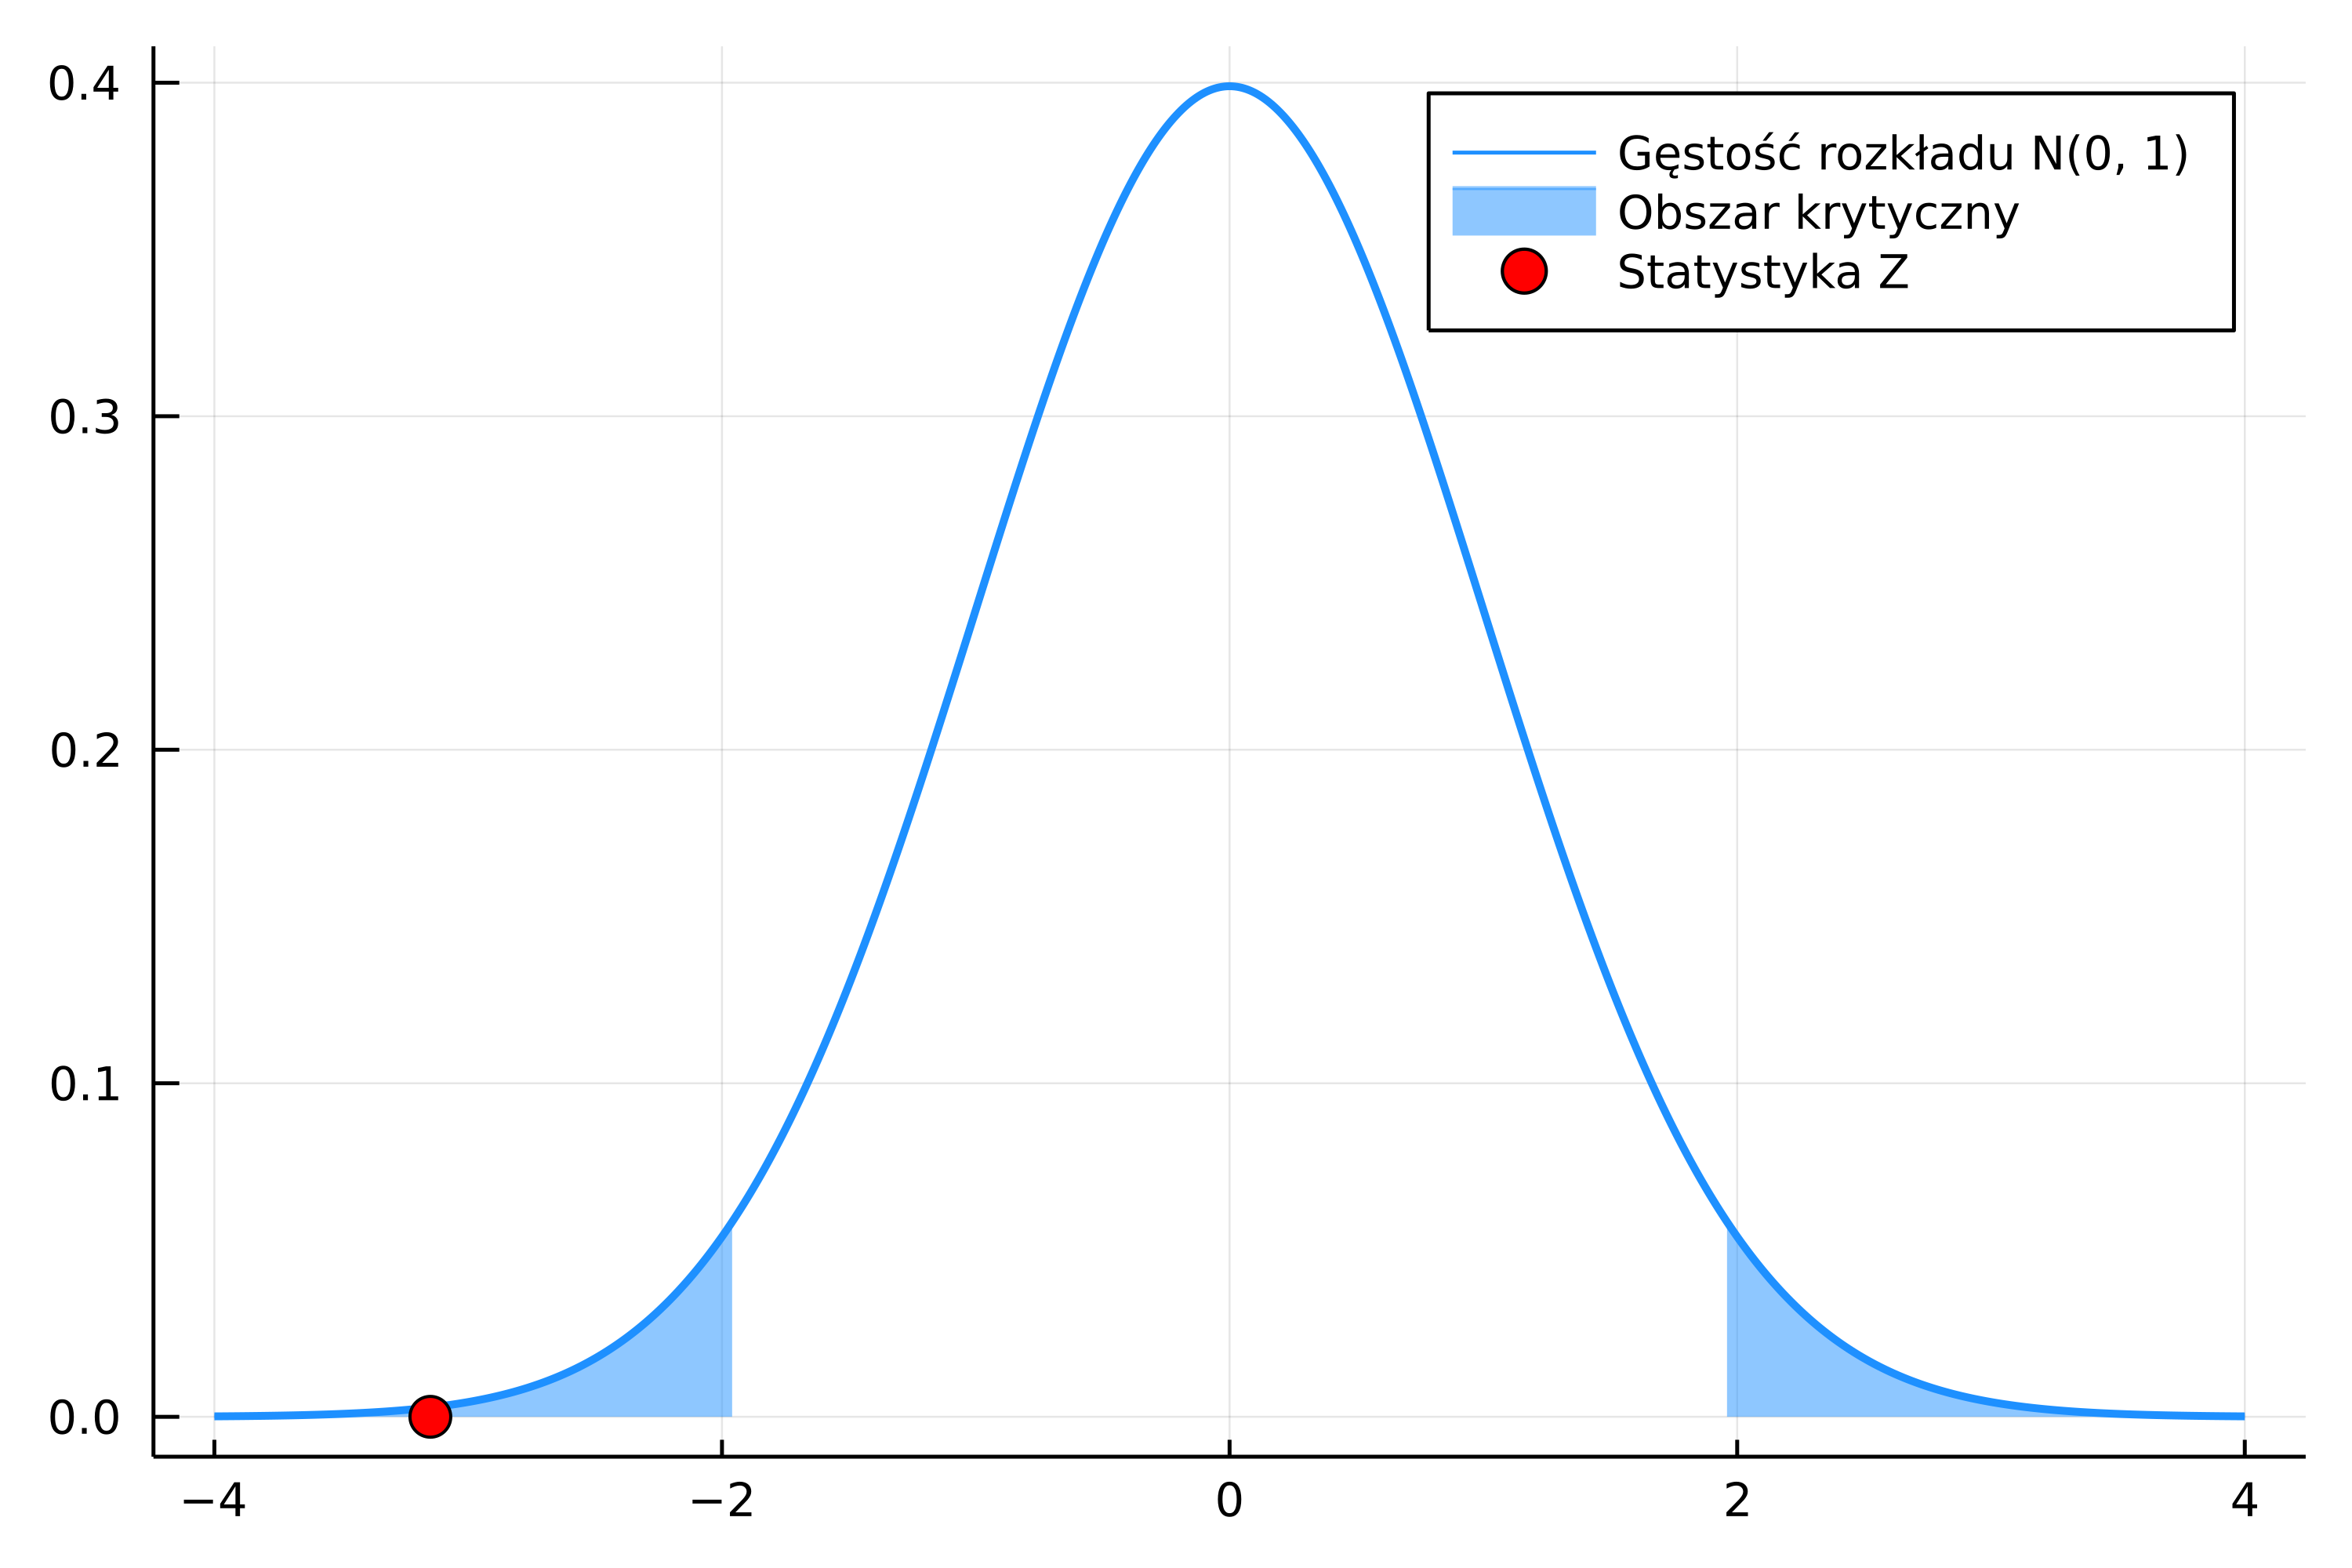
\includegraphics[scale=0.11]{images/srednia_a.png}
			\caption{Wykres gęstości rozkładu $\mathcal{N}(0, 1)$ z zaznaczonym obszarem krytycznym dla $\mathrm{H_1}: \mu \neq \mu_0$ oraz wartością statystyki $Z$.}
		\end{figure}
		
		\item {\boldmath $\mathrm{H_1}: \mu > \mu_0$}\\
		W tym przypadku obszar krytyczny ma postać
		$$ C = \left[ z_{1-\alpha} \ ; \ \infty \right) = [1.645 \ ; \ \infty), $$
		Wartość statystyki nie należy do tego przedziału, a więc przyjmujemy hipotezę zerową .
		P-wartość testu wynosi
		$$ \mathrm{P}\left(Z > -3.149 \right) \approx 0.9991. $$
		
		\begin{figure}[H]
			\centering
			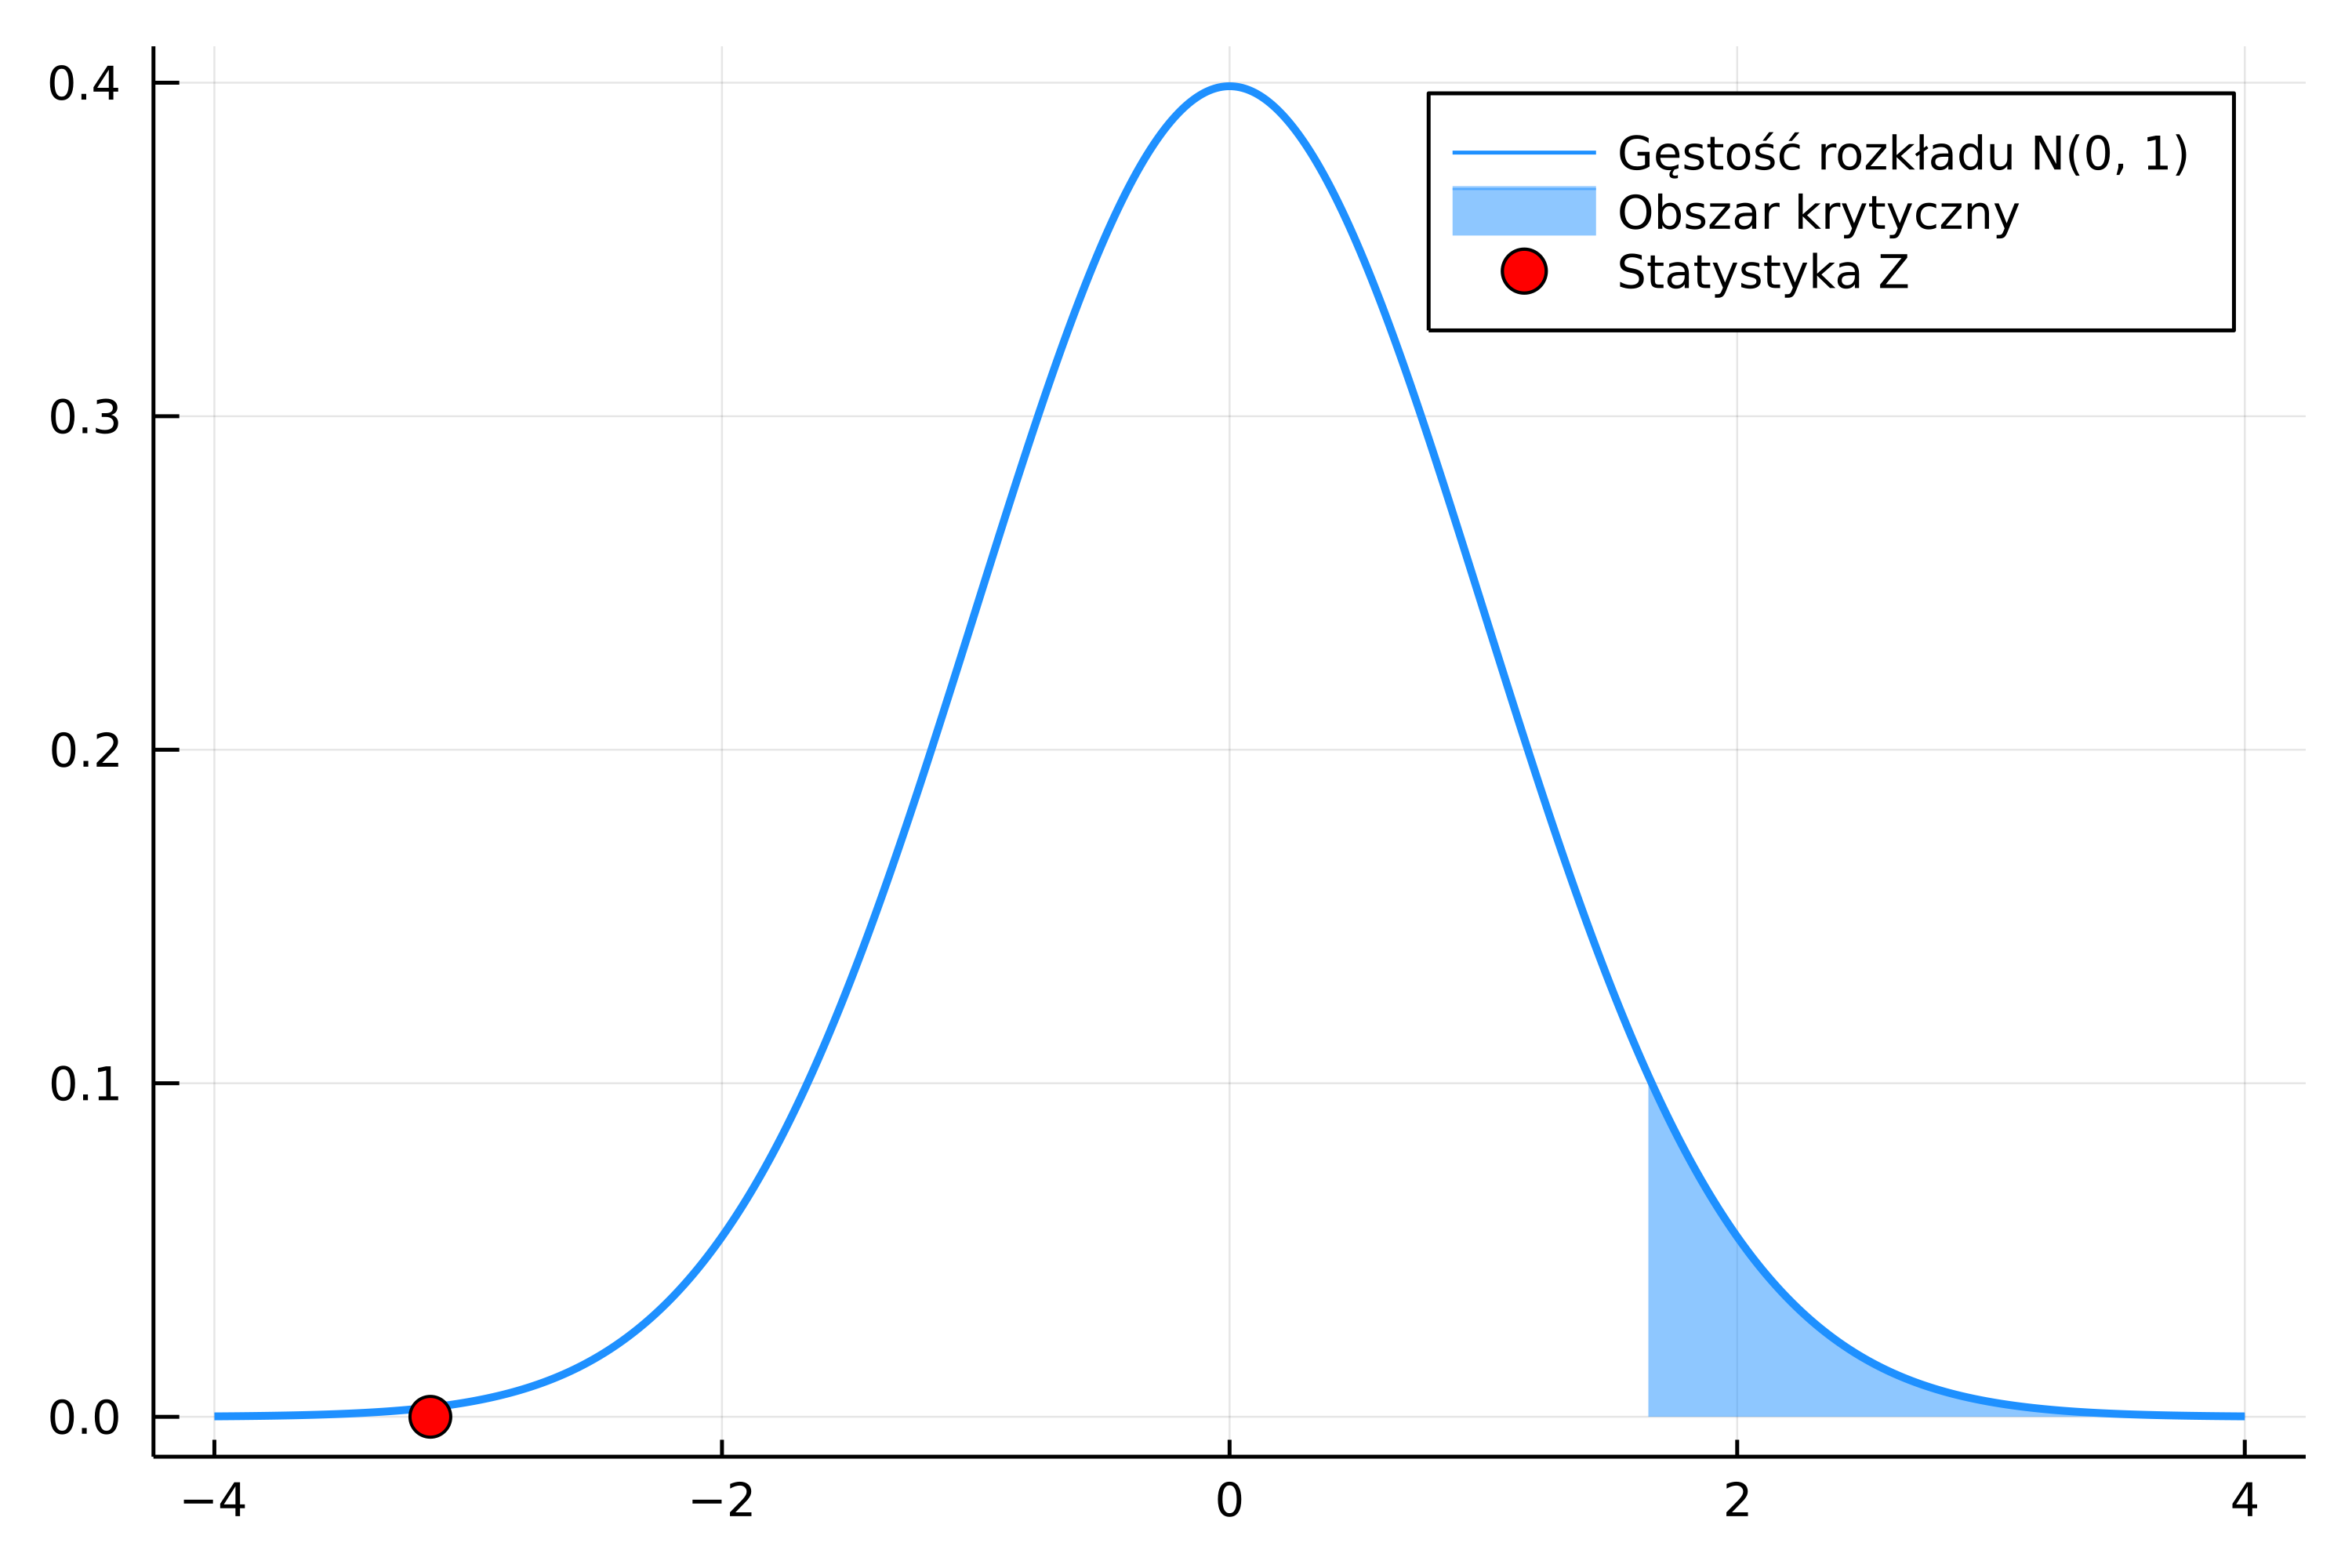
\includegraphics[scale=0.11]{images/srednia_b.png}
			\caption{Wykres gęstości rozkładu $\mathcal{N}(0, 1)$ z zaznaczonym obszarem krytycznym dla $\mathrm{H_1}: \mu > \mu_0$ oraz wartością statystyki $Z$.}
		\end{figure}
		
		\item {\boldmath $\mathrm{H_1}: \mu < \mu_0$}\\
		Obszar krytyczny w tym przypadku to
		$$ C = \left( -\infty \ ;  -z_{1-\alpha}\right] = (-\infty \ ; \ -1.645]. $$
		Wartość statystyki $Z$ mieści się w tym przedziale, zatem przyjmujemy\\ $\mathrm{H_1}$ . 
		P-wartość dla tego testu wynosi
		$$ \mathrm{P}\left(Z < -3.149 \right) \approx0.0008. $$
		
		\begin{figure}[H]
			\centering
			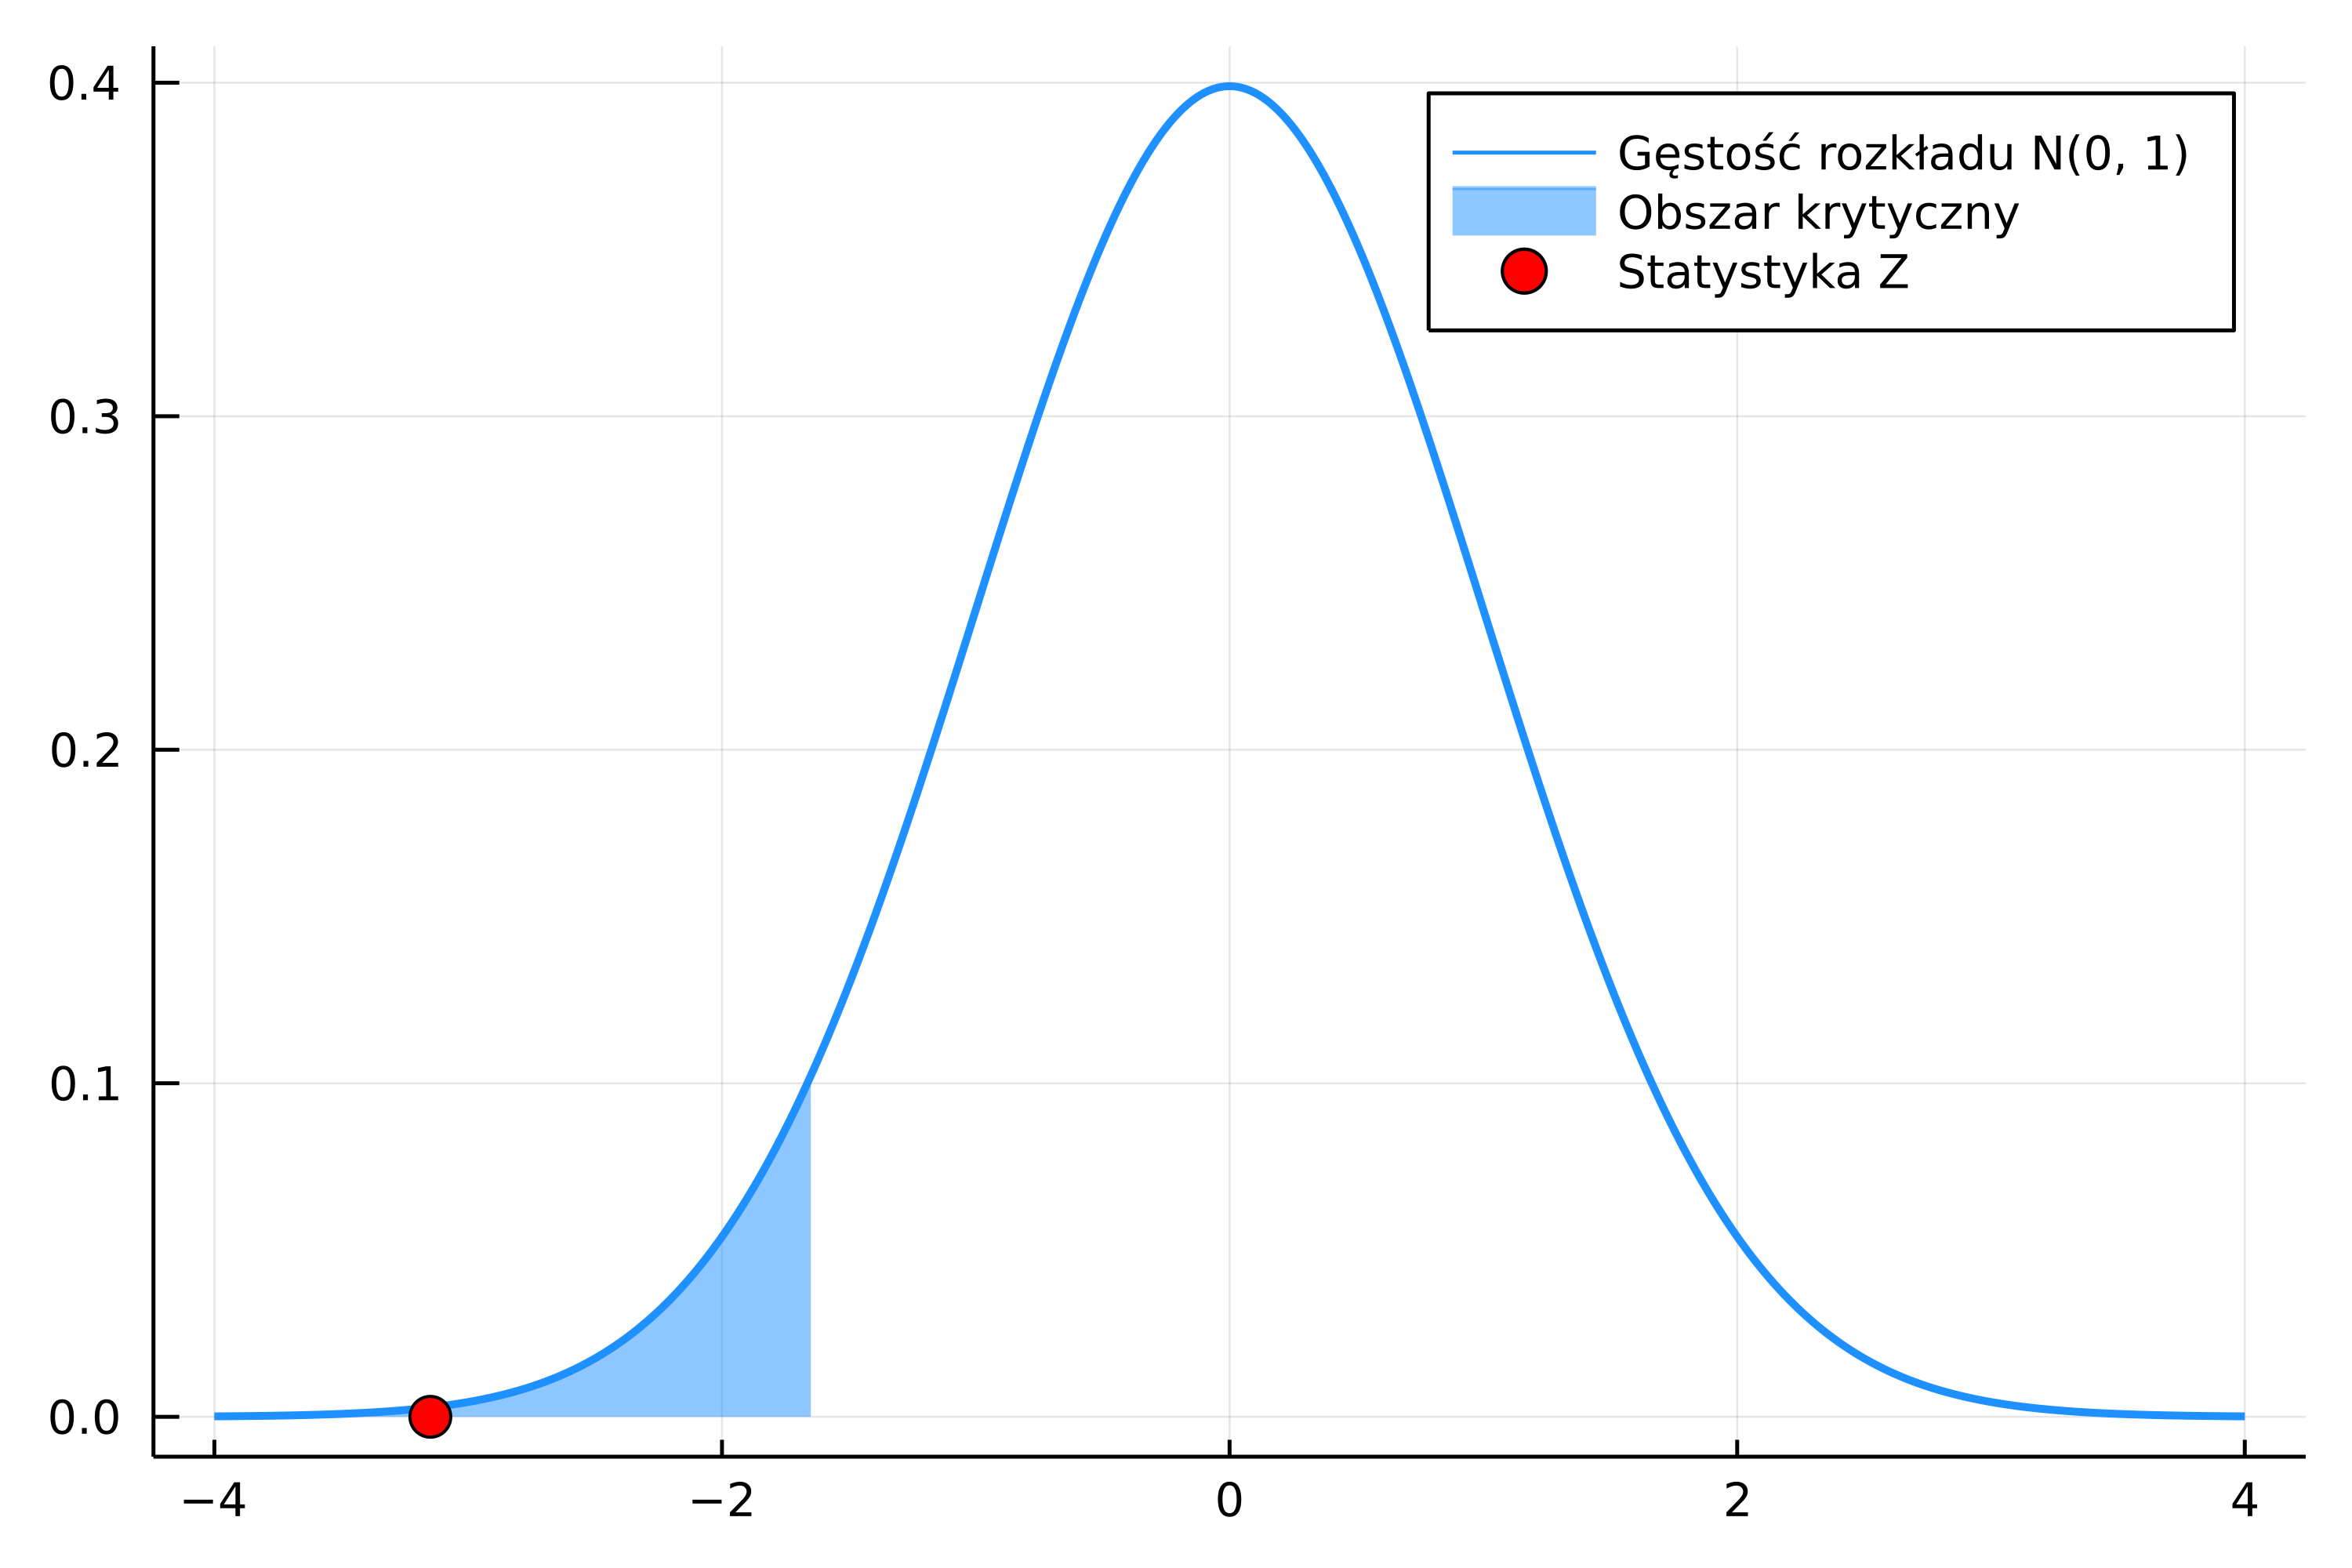
\includegraphics[scale=0.11]{images/srednia_c.png}
			\caption{Wykres gęstości rozkładu $\mathcal{N}(0, 1)$ z zaznaczonym obszarem krytycznym dla $\mathrm{H_1}: \mu < \mu_0$ oraz wartością statystyki $Z$.}
		\end{figure}
		
	\end{enumerate}

	\noindent Gdy $\alpha$ będzie równa $0,01$, to $z_{1-\frac{\alpha}{2}}=2,576$, a  $z_{1-\alpha}=2,326$, więc wraz ze zmniejszaniem $\alpha$ dojdziemy do momentu, że w każdym z podpunktów hipoteza zerowa będzie przyjmowana. 
	Gdy $\alpha$ będzie równa $0,01$, to $z_{1-\frac{\alpha}{2}}=1,645$, a  $z_{1-\alpha}=1,282$, więc wraz ze zwiększaniem $\alpha$ nic nie zmieni się w podpunkcie (a), natomiast dla $\alpha$ bliskiej 1, w podpunkcie (b), będziemy odrzucać hipotezę zerową.\vspace{2mm}
	
	\noindent Podsumowując, odrzuciliśmy hipotezę $\mathrm{H_1}:\mu > \mu_0$ przyjmując $\mathrm{H_0}$ w podpunkcie (b) oraz przyjęliśmy hipotezy alternatywne z podpunktów (a) i (c). Bardzo małe p-wartości dla tych hipotez utwierdzają nas w przekonaniu, że są one prawdziwe. Zatem z dużą dozą pewności możemy stwierdzić, że $\mu < \mu_0 = 1,5$.
	
	
	
	\section{Testowanie hipotez dotyczących wariancji}
	
	\noindent W zadaniu 2 mamy zbadać próbę $X_1, \dots, X_n$ z populacji generalnej o rozkładzie normalnym $\mathcal{N}(0,2\ , \sigma^2)$. Dane dostępne są na stronie \cite{dane2}. Długość próby wynosi $n = 1000$. Oznaczmy $\mu = 0,2$ oraz $\sigma_0^2 = 1,5$. Naszym zadaniem jest zweryfikowanie hipotezy zerowej
	$$ \mathrm{H_0}: \sigma^2 = \sigma_0^2 = 1,5 $$
	na poziomie istotności $\alpha = 0,05$. W tym celu konstruujemy statystykę
	$$ \chi^2 = \frac{nS^2}{\sigma_0^2}, $$
	gdzie
	$$ S^2 = \frac{1}{n} \sum_{i=1}^n (X_i - \mu)^2 $$
	jest nieobciążonym estymatorem wariancji. Zauważmy, że
	$$ \chi^2 = \frac{nS^2}{\sigma_0^2} = \sum_{i=1}^n \left(\frac{X_i - \mu}{\sigma_0}\right)^2 \sim \chi^2(n), $$
	pod warunkiem zachodzenia $\mathrm{H_0}$. Jeśli $\mathrm{H_0}$ jest fałszywa, statystyka $\chi$ będzie miała tendencję do przyjmowania dużych lub małych wartości. Dla naszych danych wartość statystyki wynosi {\boldmath$1112,58$}. Hipotezę zerową będziemy testować naprzeciw trzem hipotezom alternatywnym.
	
	\begin{enumerate}[label=(\textbf{\alph*})]
		
		\item {\boldmath $\mathrm{H_1}: \sigma^2 \neq \sigma_0^2$}\\
		Definiujemy obszar krytyczny jako przedział
		$$ C = \left( -\infty \ ; \ x^2_{\frac{\alpha}{2}, n} \right] \cup \left[ x^2_{1 - \frac{\alpha}{2}, n} \ ; \ \infty \right), $$
		gdzie  $x^2_{\frac{\alpha}{2}, n}$ i $x^2_{1 - \frac{\alpha}{2}, n}$ są kwantylami odpowiednio rzędu $\frac{\alpha}{2}$ i $1 - \frac{\alpha}{2}$ rozkładu $\chi^2$ z $n$ stopniami swobody. Jeśli $\mathrm{H_0}$ jest prawdziwa, to prawdopodobieństwo, że wartość statystyki będzie mieściła się w w przedziale $C$, wynosi \mbox{$\alpha = 0,05$}. Dla naszych danych
		$$ C = (-\infty \ ; \ 914,25] \cup [1089,53 \ ; \ \infty), $$
		a więc wartość statystyki $\chi$ mieści się w tym przedziale, zatem odrzucamy hipotezę zerową i przyjmujemy hipotezę $\mathrm{H_1}$.
		P-wartość tego testu wynosi
		$$ 2\cdot\mathrm{P}\left(\chi^2 > 1112,58 \right) \approx 0,0145. $$
		
		\begin{figure}[H]
			\centering
			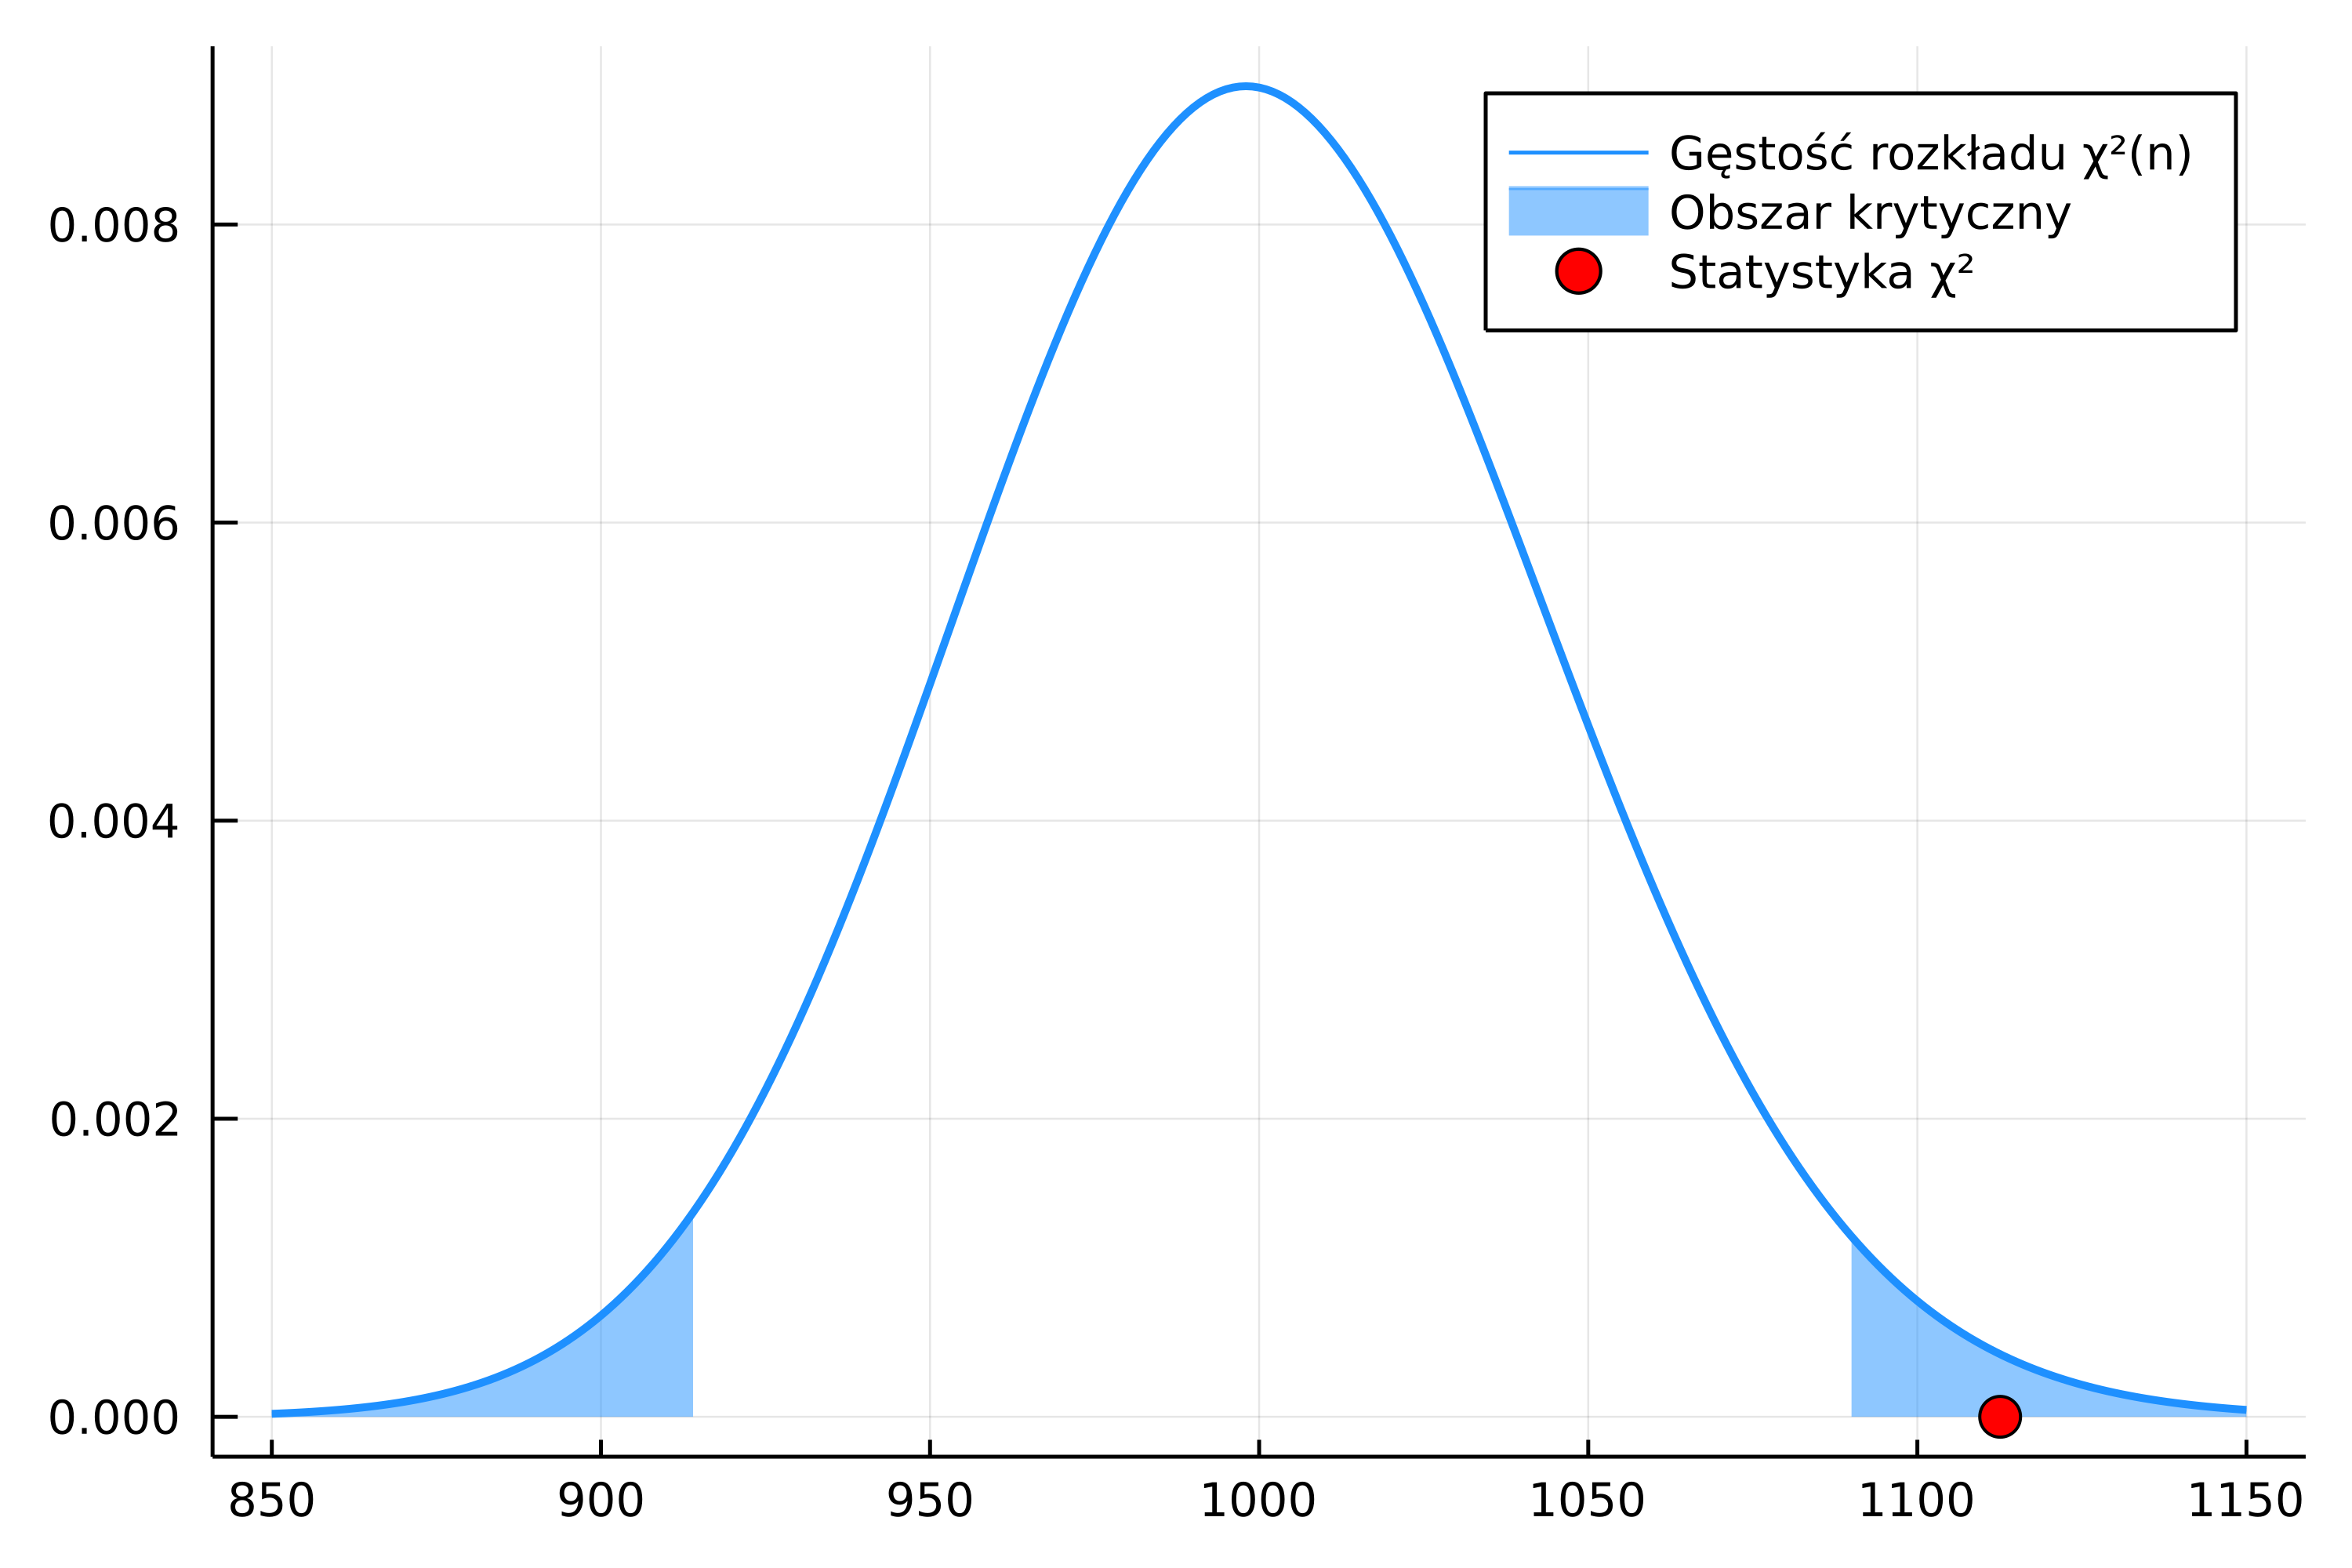
\includegraphics[scale=0.11]{images/wariancja_a.png}
			\caption{Wykres gęstości rozkładu $\chi^2(n)$ z zaznaczonym obszarem krytycznym dla $\mathrm{H_1}: \sigma^2 \neq \sigma_0^2$ oraz wartością statystyki $\chi^2$.}
		\end{figure}
		
		\item {\boldmath $\mathrm{H_1}: \sigma^2 > \sigma_0^2$}\\
		W tym przypadku obszar krytyczny ma postać
		$$ C = \left[ x^2_{1 - \alpha, n} \ ; \ \infty \right) = [1074,68 \ ; \ \infty), $$
		czyli również wartość statystyki należy do tego przedziału, a więc przyjmujemy hipotezę $\mathrm{H_1}$.
		P-wartość testu wynosi
		$$ \mathrm{P}\left(\chi^2 > 1112,58 \right) \approx 0,0073. $$
		
		\begin{figure}[H]
			\centering
			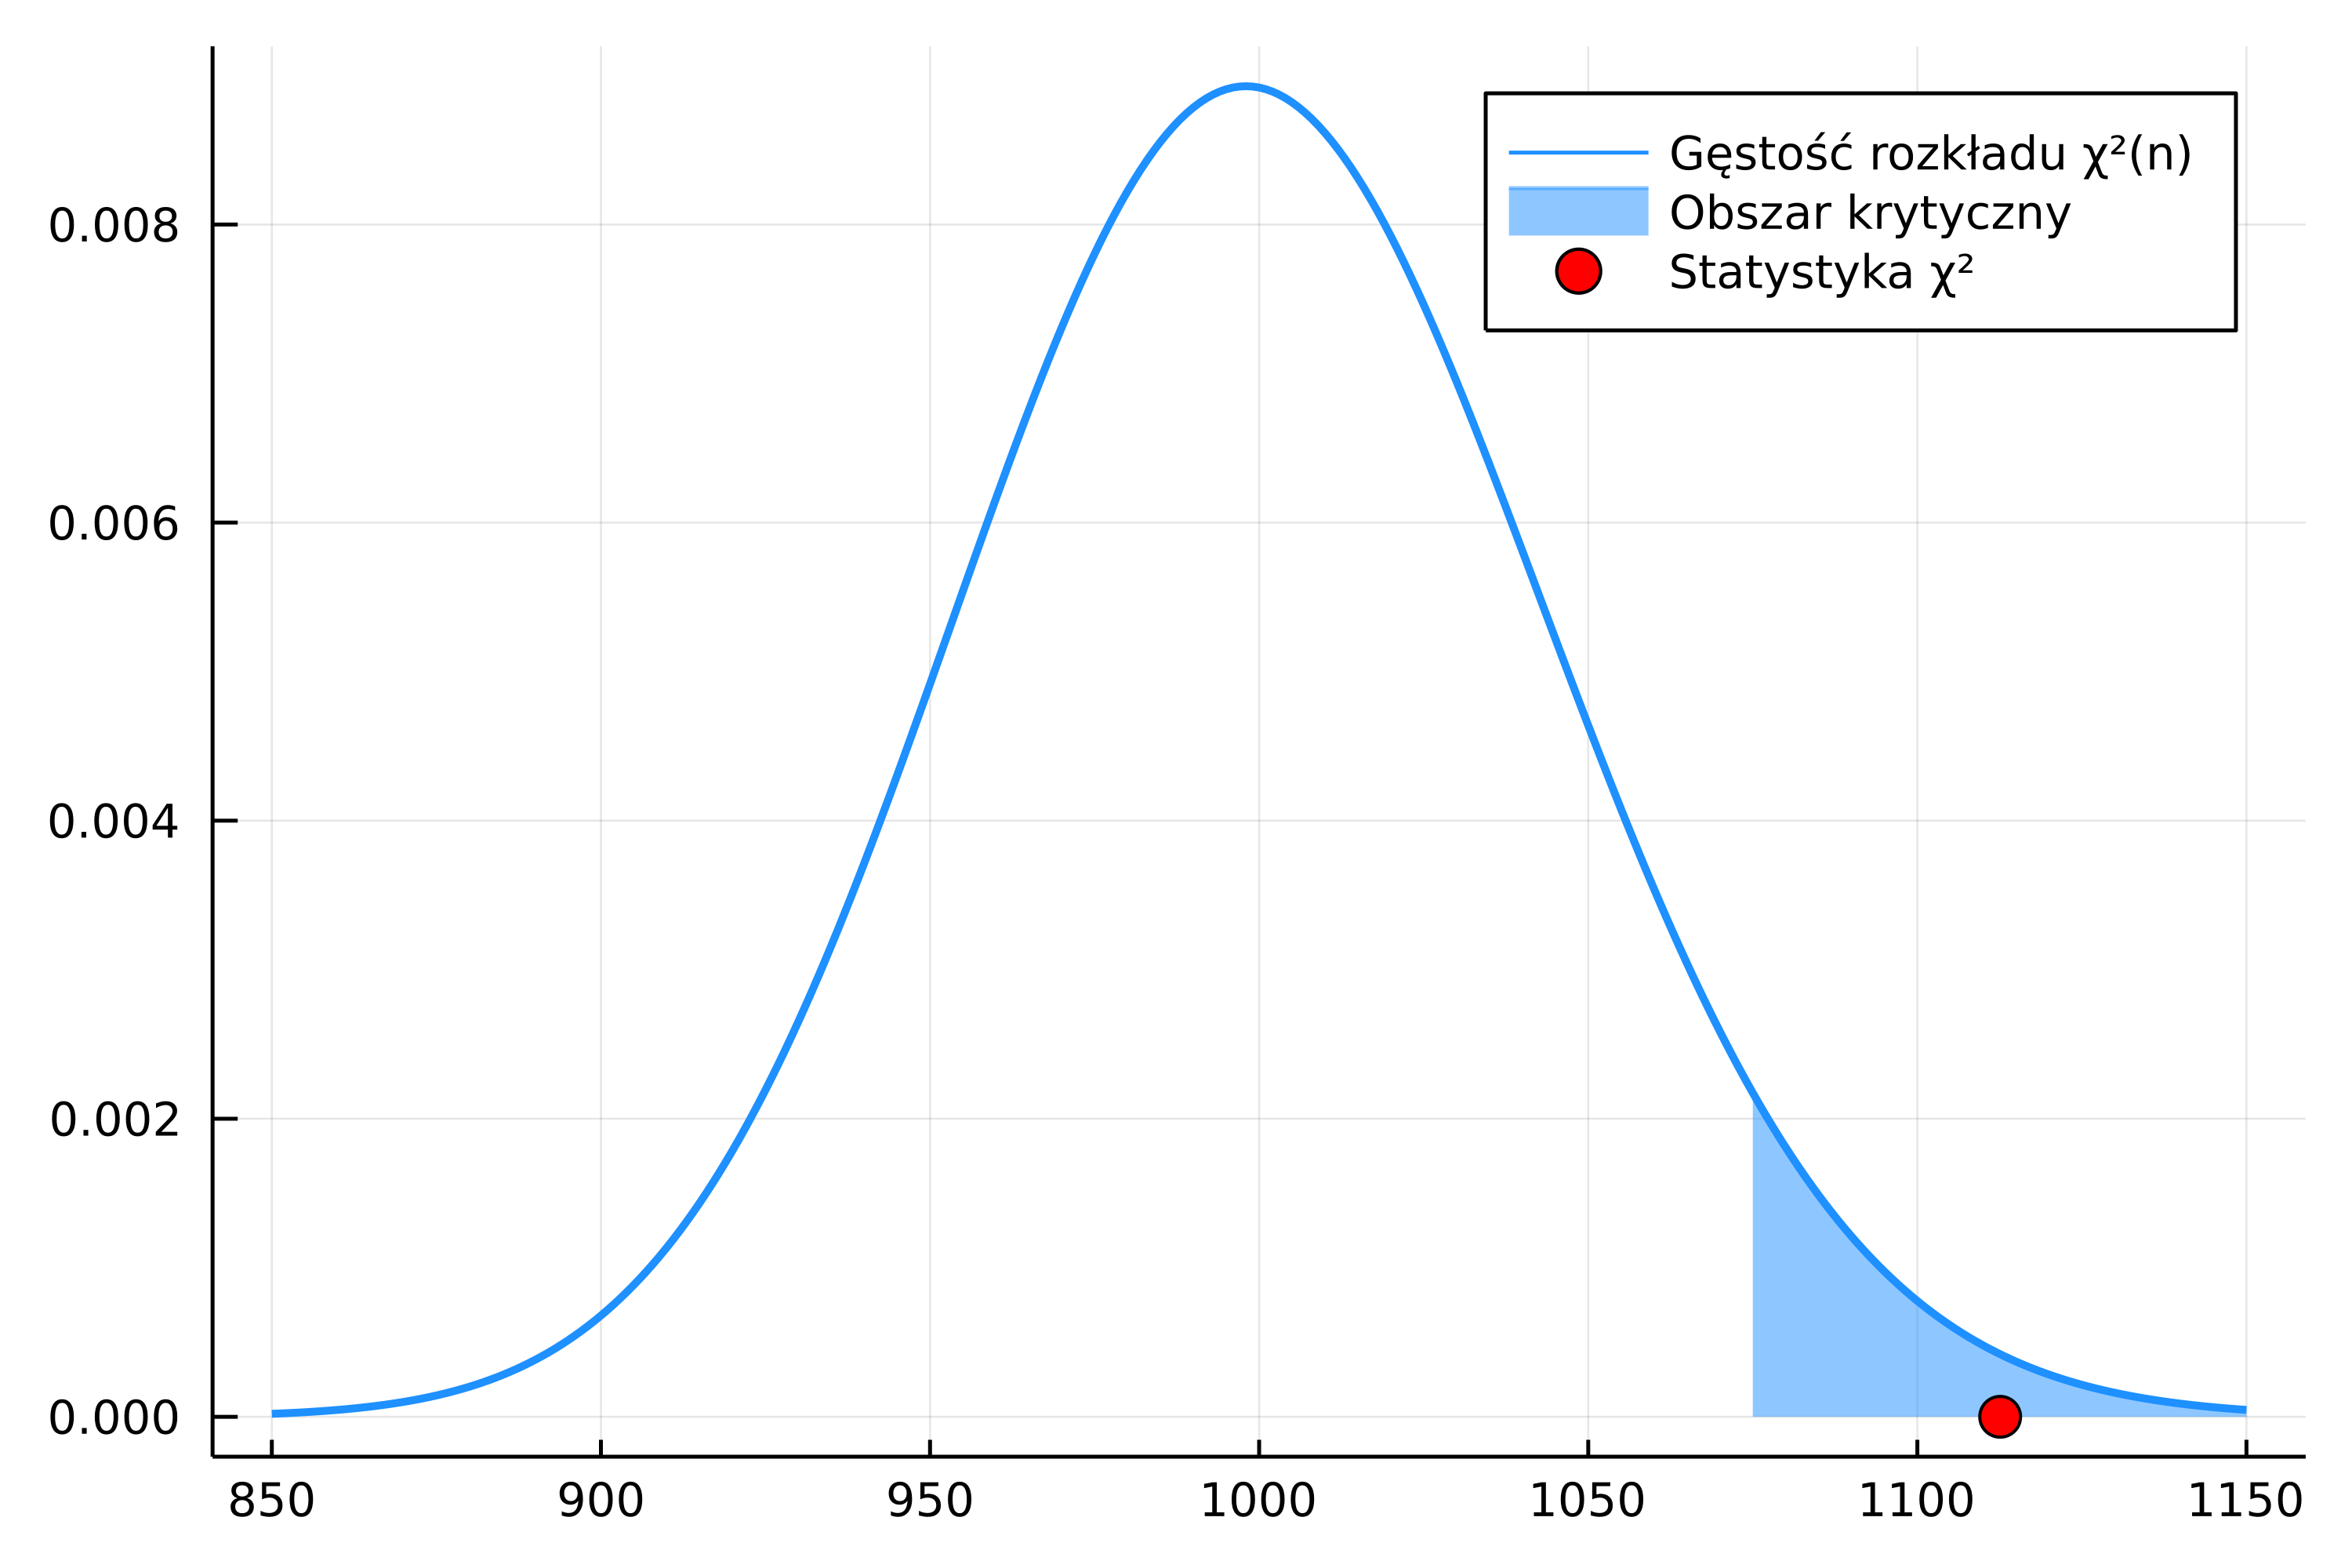
\includegraphics[scale=0.11]{images/wariancja_b.png}
			\caption{Wykres gęstości rozkładu $\chi^2(n)$ z zaznaczonym obszarem krytycznym dla $\mathrm{H_1}: \sigma^2 > \sigma_0^2$ oraz wartością statystyki $\chi^2$.}
		\end{figure}
		
		\item {\boldmath $\mathrm{H_1}: \sigma^2 < \sigma_0^2$}\\
		Obszar krytyczny w tym przypadku to
		$$ C = \left( -\infty \ ; \ x^2_{\alpha, n} \right] = (-\infty \ ; \ 927,6]. $$
		Wartość statystyki $\chi^2$ nie mieści się w tym przedziale, zatem przyjmujemy hipotezę zerową. 
		P-wartość dla tego testu wynosi
		$$ \mathrm{P}\left(\chi^2 < 1112,58 \right) \approx 0,9927. $$
		
		\begin{figure}[H]
			\centering
			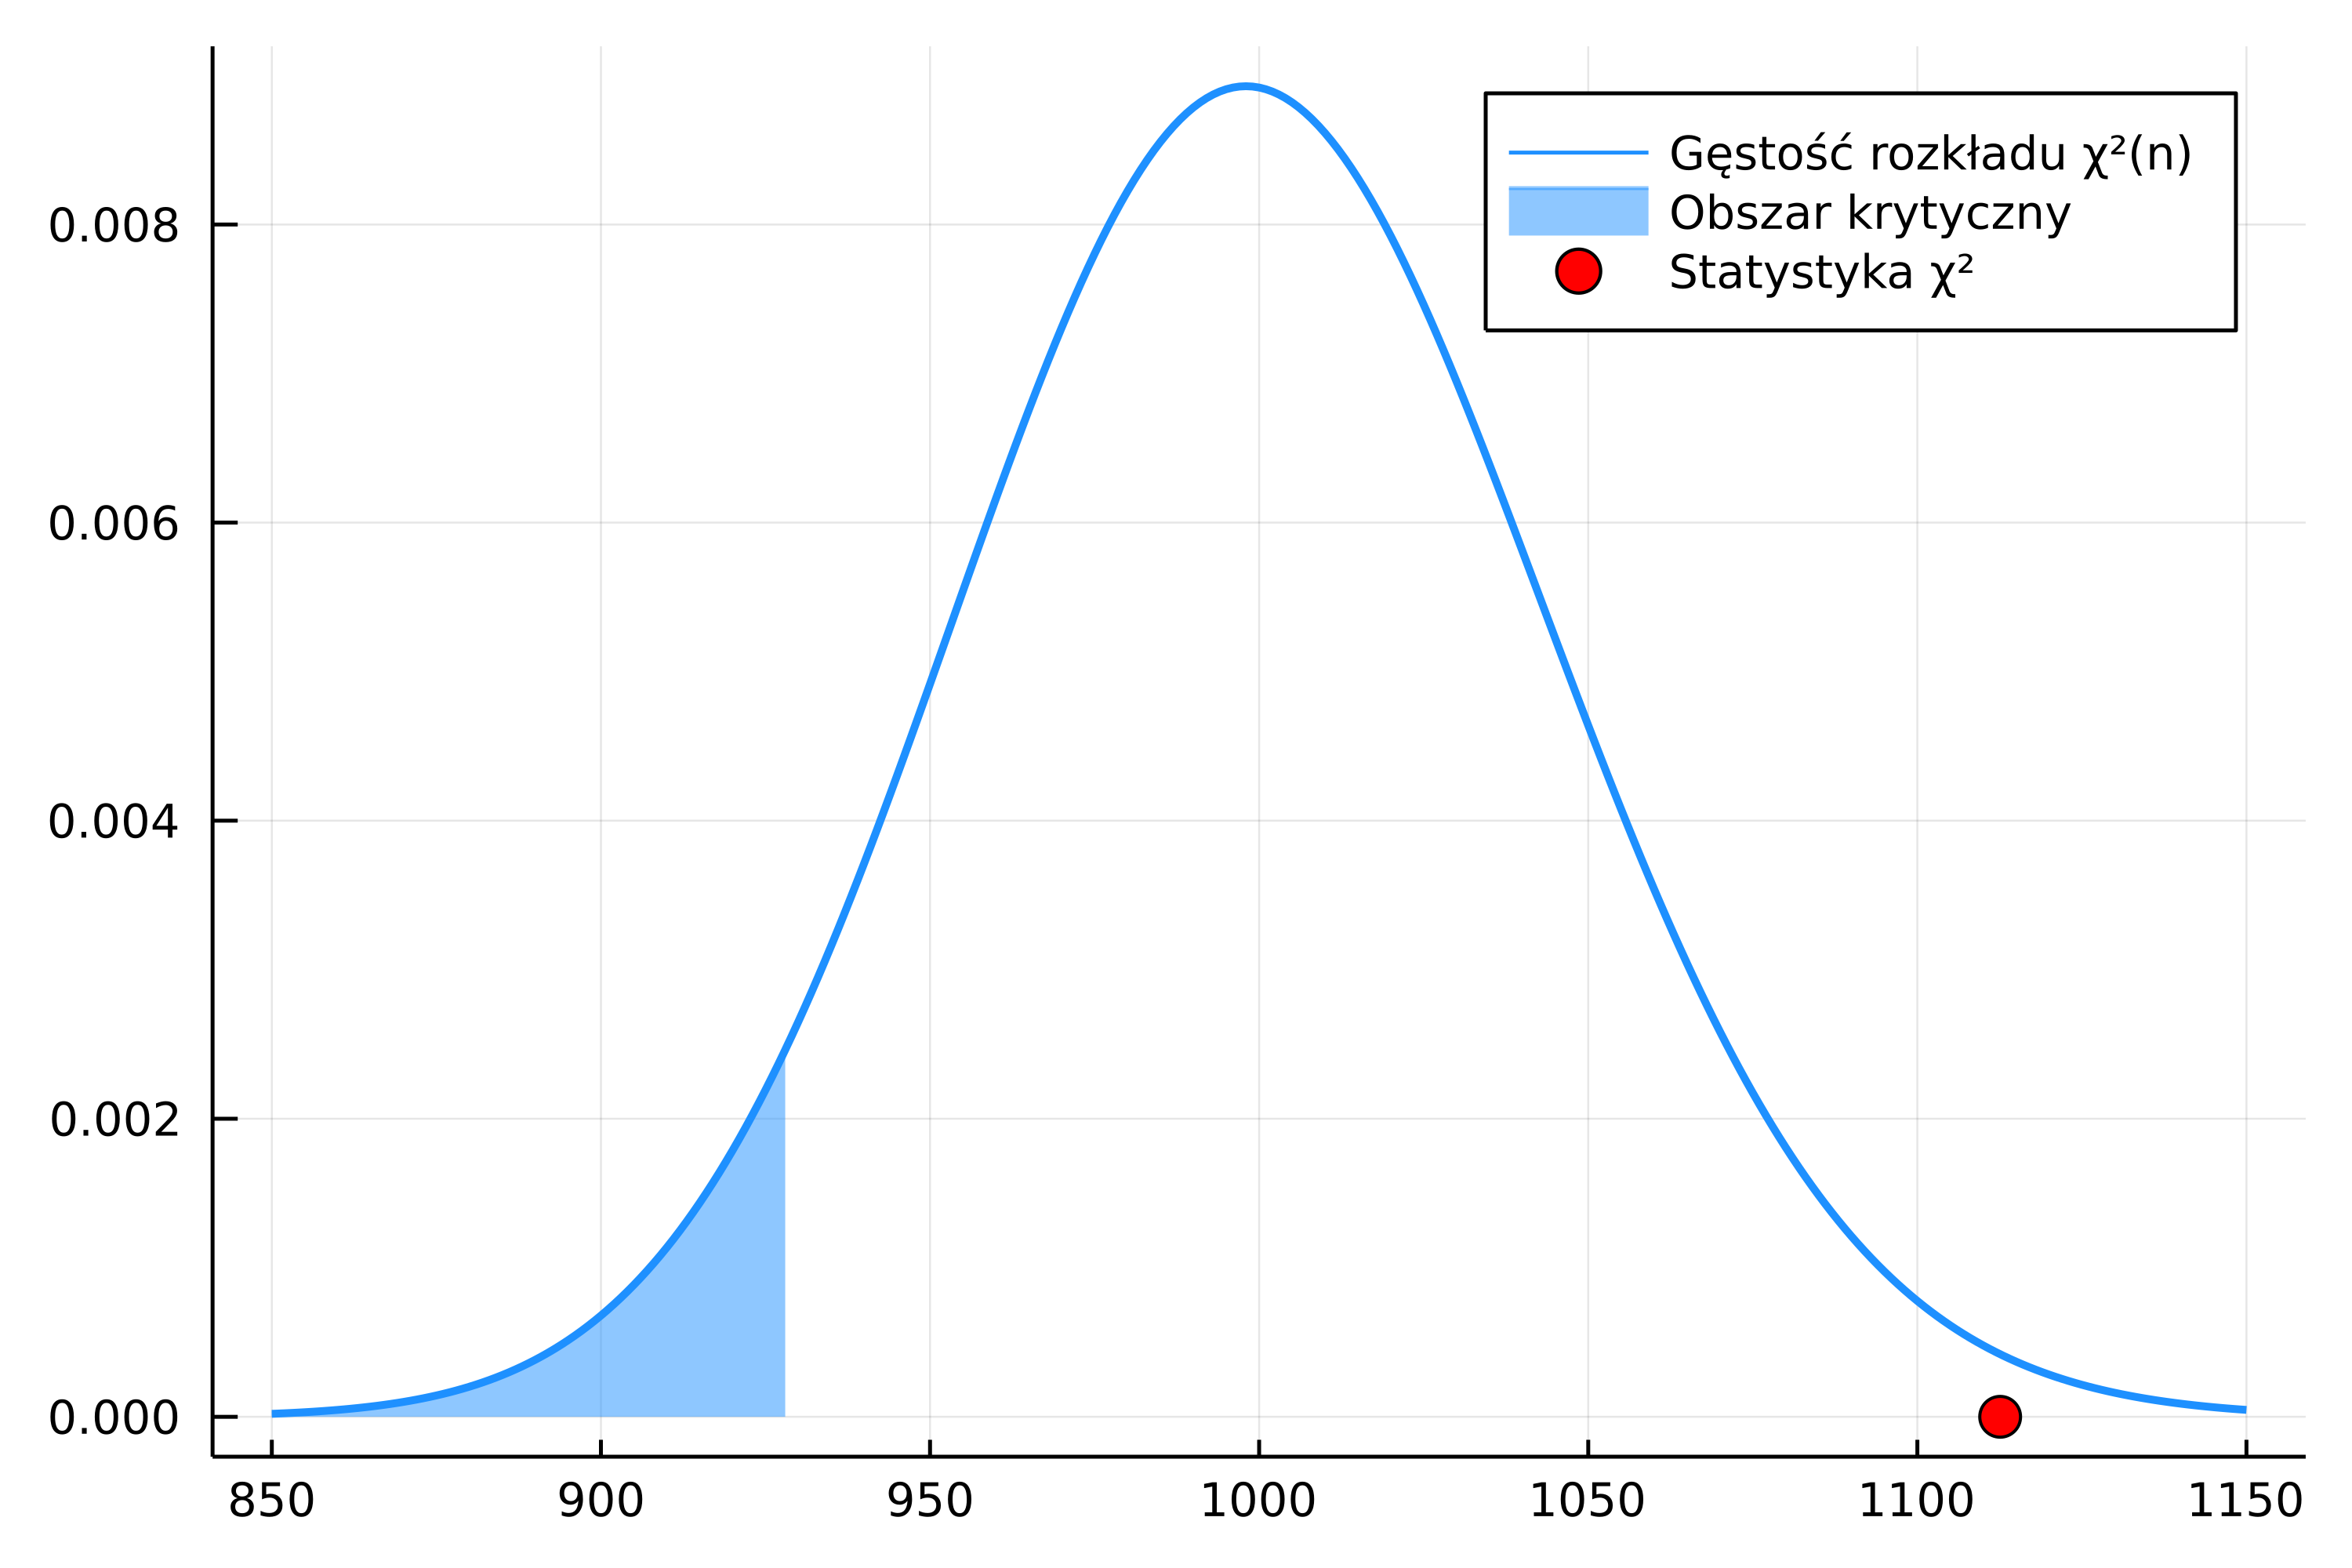
\includegraphics[scale=0.11]{images/wariancja_c.png}
			\caption{Wykres gęstości rozkładu $\chi^2(n)$ z zaznaczonym obszarem krytycznym dla $\mathrm{H_1}: \sigma^2 < \sigma_0^2$ oraz wartością statystyki $\chi^2$.}
		\end{figure}
		
	\end{enumerate}

	\noindent Podobnie, jak w przypadku hipotez dotyczących $\mu$, gdy będziemy zmniejszać wartość $\alpha$, będzie zmniejszał się obszar krytyczny, a więc w pewnym momencie dla każdego przypadku hipoteza zerowa będzie akceptowana. Jeśli z kolei zwiększymy wartość $\alpha$, doprowadzimy do tego, że poza $\mathrm{H_1}$ z podpunktów (a) i (b) zostanie przyjęta także hipoteza alternatywna z podpunktu (c), jednak wartość ta musiałaby być równa aż 0,9927. \vspace{2mm}
	
	\noindent Podsumowując, odrzuciliśmy hipotezę $\mathrm{H_1}:\sigma^2 < \sigma_0^2$ przyjmując $\mathrm{H_0}$ w podpunkcie (c) oraz przyjęliśmy hipotezy alternatywne z podpunktów (a) i (b). Małe p-wartości dla tych hipotez wyraźnie sugerują, że są one prawdziwe. Zatem możemy stwierdzić, że z dużym prawdopodobieństwem $\sigma^2 > \sigma_0^2 = 1,5$.
	
	
	
	\section{Wyznaczenie symulacyjnie prawdopodobieństwa popełnienia błędów I i II rodzaju}
	
	\noindent Zadanie 3 polega na obliczeniu metodą Monte Carlo prawdopodobieństwa popełnienia błędów I i II rodzaju dla hipotez z dwóch poprzednich zadań. W przypadku hipotez dotyczących $\mu$ musimy wygenerować $N = 1000$ prób z rozkładu normalnego $\mathcal{N}(\mu_0, \sigma^2)$ o długości $n = 1000$. Z każdej próby wyliczamy statystykę $Z$, a więc otrzymujemy $Z_1, \dots, Z_n$. Następnie definiujemy zbiór
	$$ K_I = \left\{ Z_i: Z_i \in C, \ i = 1,\dots,n \right\}, $$
	gdzie $C$ jest obszarem krytycznym dla danej hipotezy alternatywnej. Prawdopodobieństwo popełnienia błędu I rodzaju wynosi
	$$ p_I = \frac{\#K_I}{N}. $$
	Jeżeli chcemy obliczyć prawdopodobieństwo popełnienia błędu II rodzaju, wykonujemy te same kroki, tylko tym razem generujemy próby z rozkładu $\mathcal{N}(\mu_0 + \theta, \sigma^2)$, $\theta \neq 0$. Definiujemy zbiór
	$$ K_{II} = \left\{ Z_i: Z_i \notin C, \ i = 1,\dots,n \right\}. $$
	Szukane prawdopodobieństwo jest równe
	$$ p_{II} = \frac{\#K_{II}}{N}. $$
	W przypadku hipotez dotyczących wariancji postępujemy analogicznie, tylko zamiast statystyki $Z$ obliczamy statystykę $\chi^2$.
	
	\noindent Gdy znamy już prawdopodobieństwo popełnienia błędu II rodzaju, w prosty sposób możemy policzyć moc testu, ponieważ jest ona równa $1 - p_{II}$. Poniżej widoczne są wyniki przeprowadzonych symulacji.\vspace{4mm}
	
	\begin{figure}[H]
		\centering
		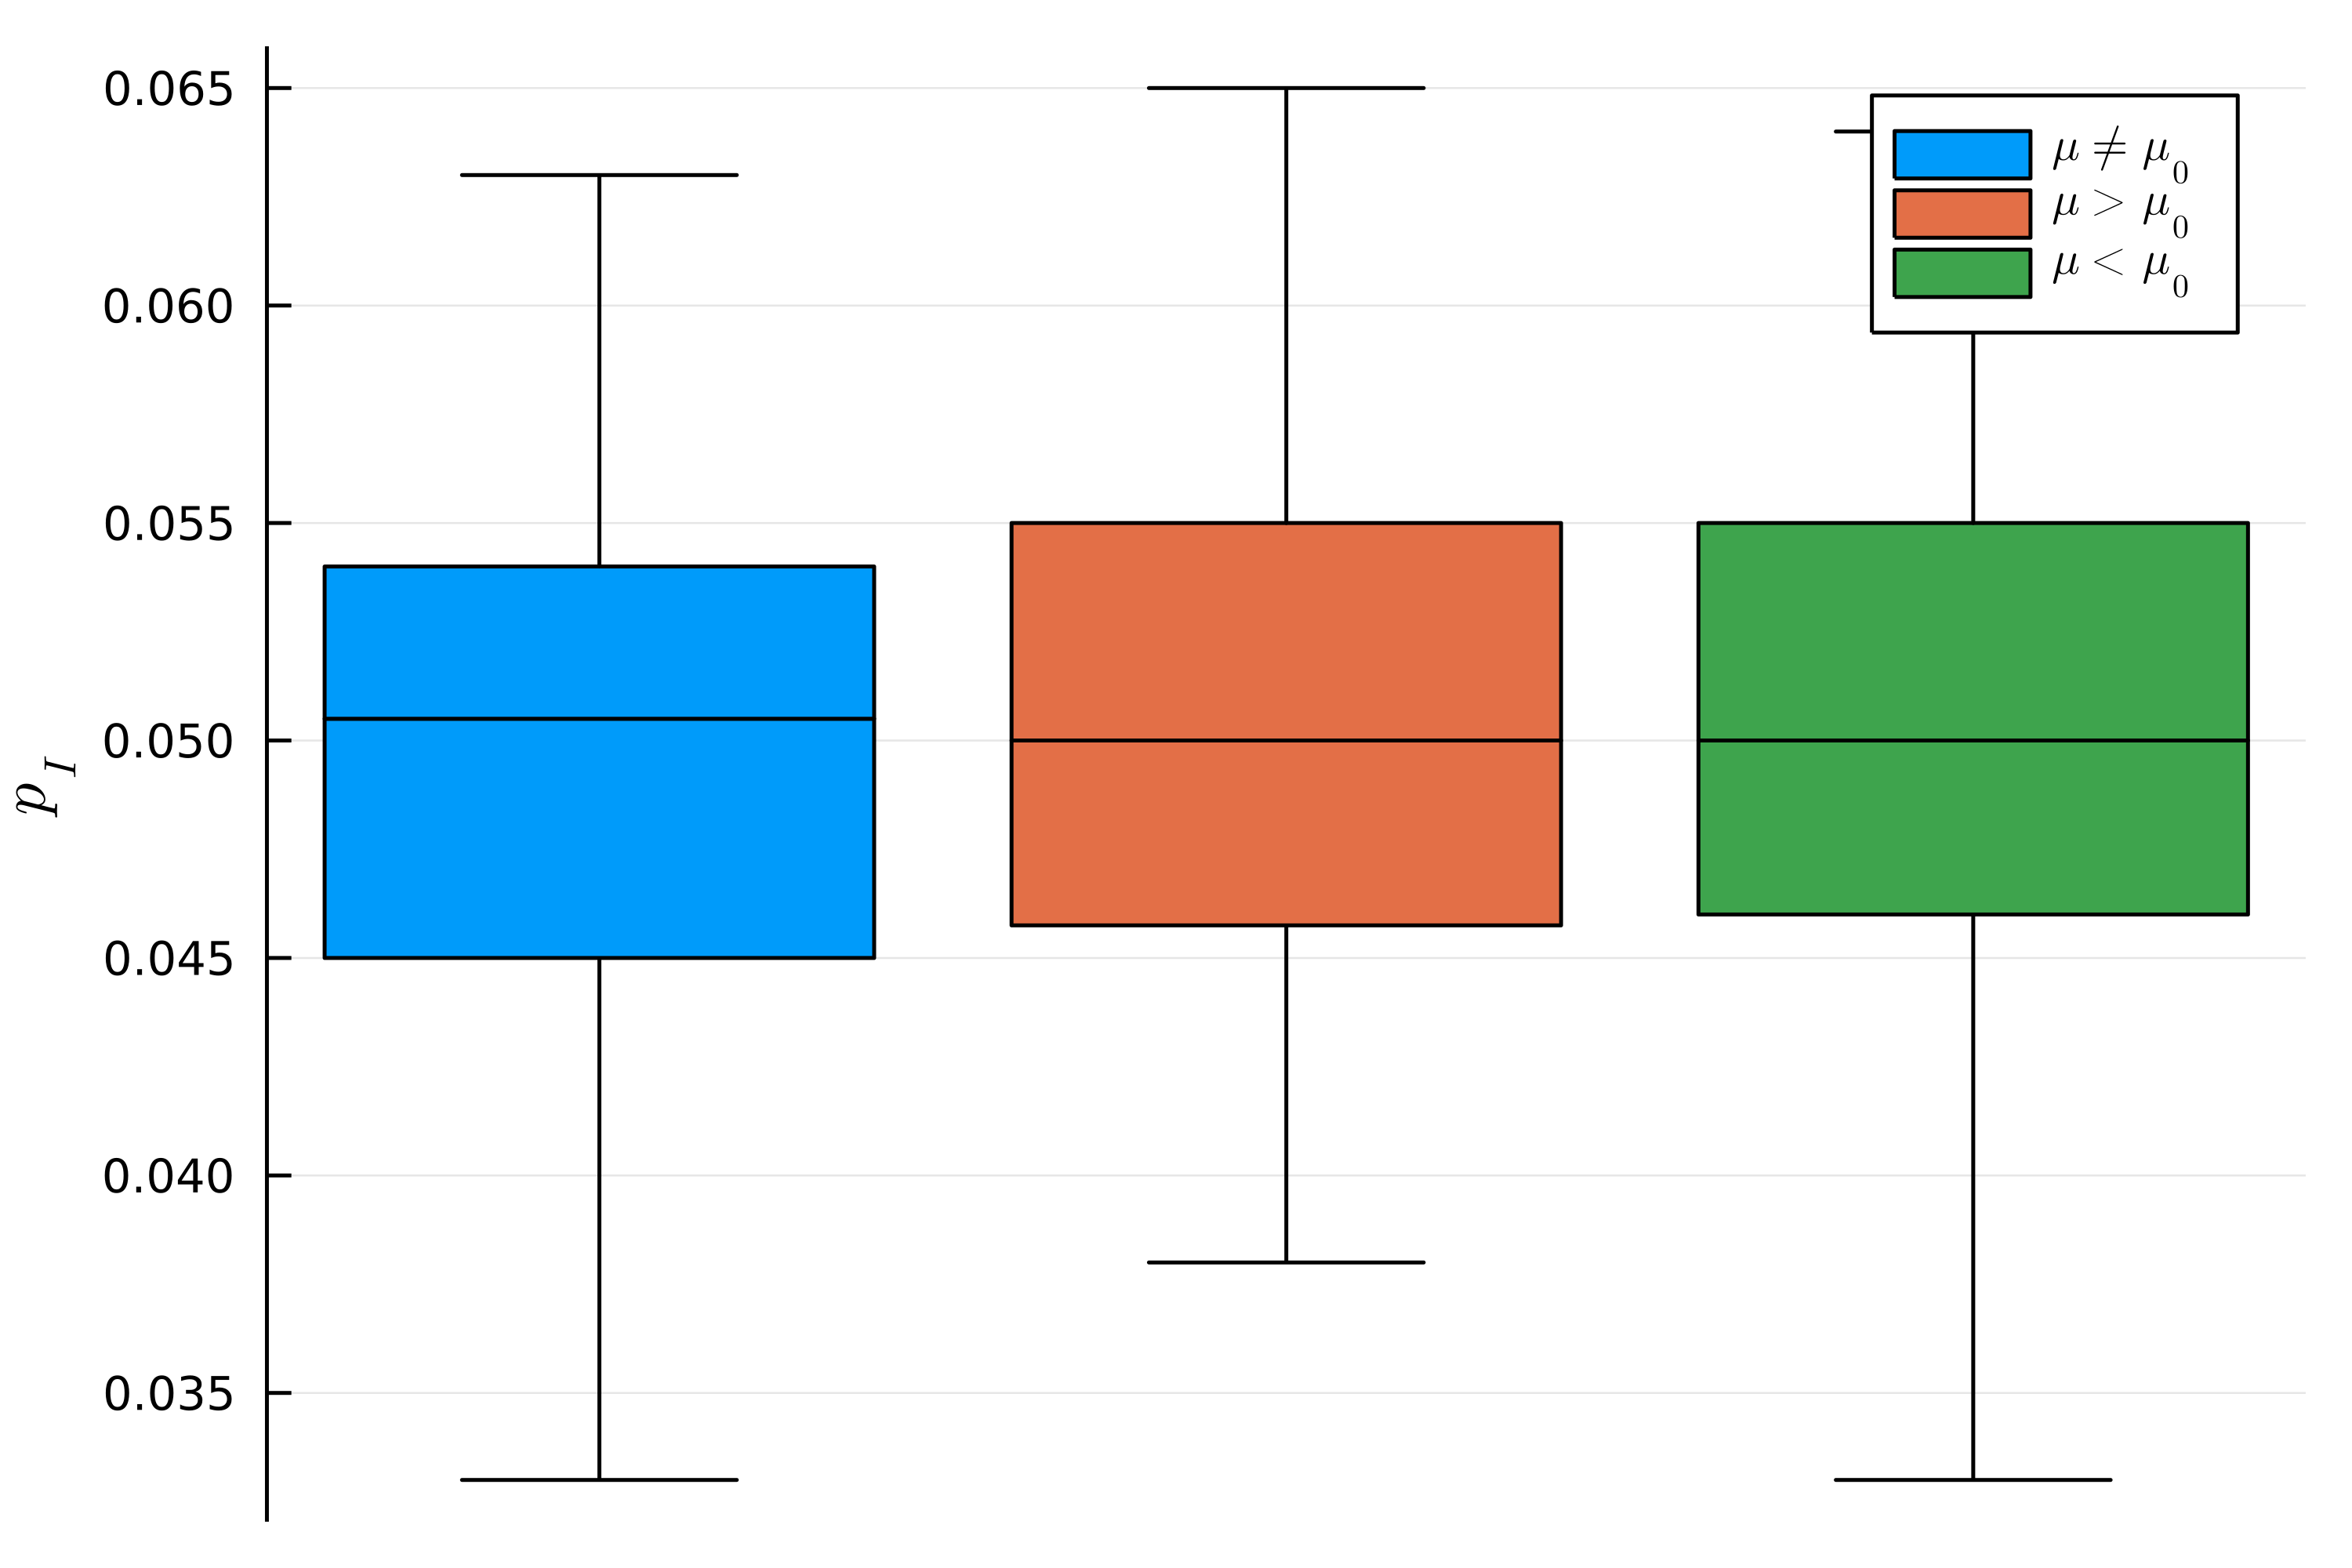
\includegraphics[scale=0.11]{images/boxplot_srednia.png}
		\caption{Wykresy pudełkowe 100 wysymulowanych wartości prawdopodobieństwa popełnienia błędu I rodzaju dla każdej z hipotez dotyczących parametru $\mu$ w pierwszym zadaniu.}
	\end{figure}

	\begin{table}[H]
		\centering
		\begin{tabular}{ |c|c|c|c| } 
			\hline
			\vphantom{ $1^{1^1}$} $\mu$ \vphantom{ $1^{1^{1^1}}$} & $\mu \neq \mu_0$ & $\mu > \mu_0$ & $\mu < \mu_0$ \\\hline
			1,47 & 0,457 & -- & 0,331 \\\hline
			1,48 & 0,730 & -- & 0,621 \\\hline
			1,49 & 0,891 & -- & 0,815 \\\hline
			1,51 & 0,895 & 0,835 & -- \\\hline
			1,52 & 0,690 & 0,575 & -- \\\hline
			1,53 & 0,418 & 0,304 & -- \\\hline
		\end{tabular}
		\caption{Wartości prawdopodobieństwa popełnienia błędu II rodzaju dla podanych w 2. zadaniu hipotez alternatywnych, wyznaczone symulacyjnie dla różnych wartości $\mu$.}
	\end{table}
	
	\begin{table}[H]
		\centering
		\begin{tabular}{ |c|c|c|c| } 
			\hline
			\vphantom{ $1^{1^1}$} $\mu$ \vphantom{ $1^{1^{1^1}}$} & $\mu \neq \mu_0$ & $\mu > \mu_0$ & $\mu < \mu_0$ \\\hline
			1,47 & 0,543 & -- & 0,669 \\\hline
			1,48 & 0,270 & -- & 0,379 \\\hline
			1,49 & 0,109 & -- & 0,185 \\\hline
			1,51 & 0,105 & 0,165 & -- \\\hline
			1,52 & 0,310 & 0,425 & -- \\\hline
			1,53 & 0,582 & 0,696 & -- \\\hline
		\end{tabular}
		\caption{Wartości mocy testu dla podanych w 2. zadaniu hipotez alternatywnych, wyznaczone symulacyjnie dla różnych wartości $\mu$.}
	\end{table}
	
	\begin{figure}[H]
		\centering
		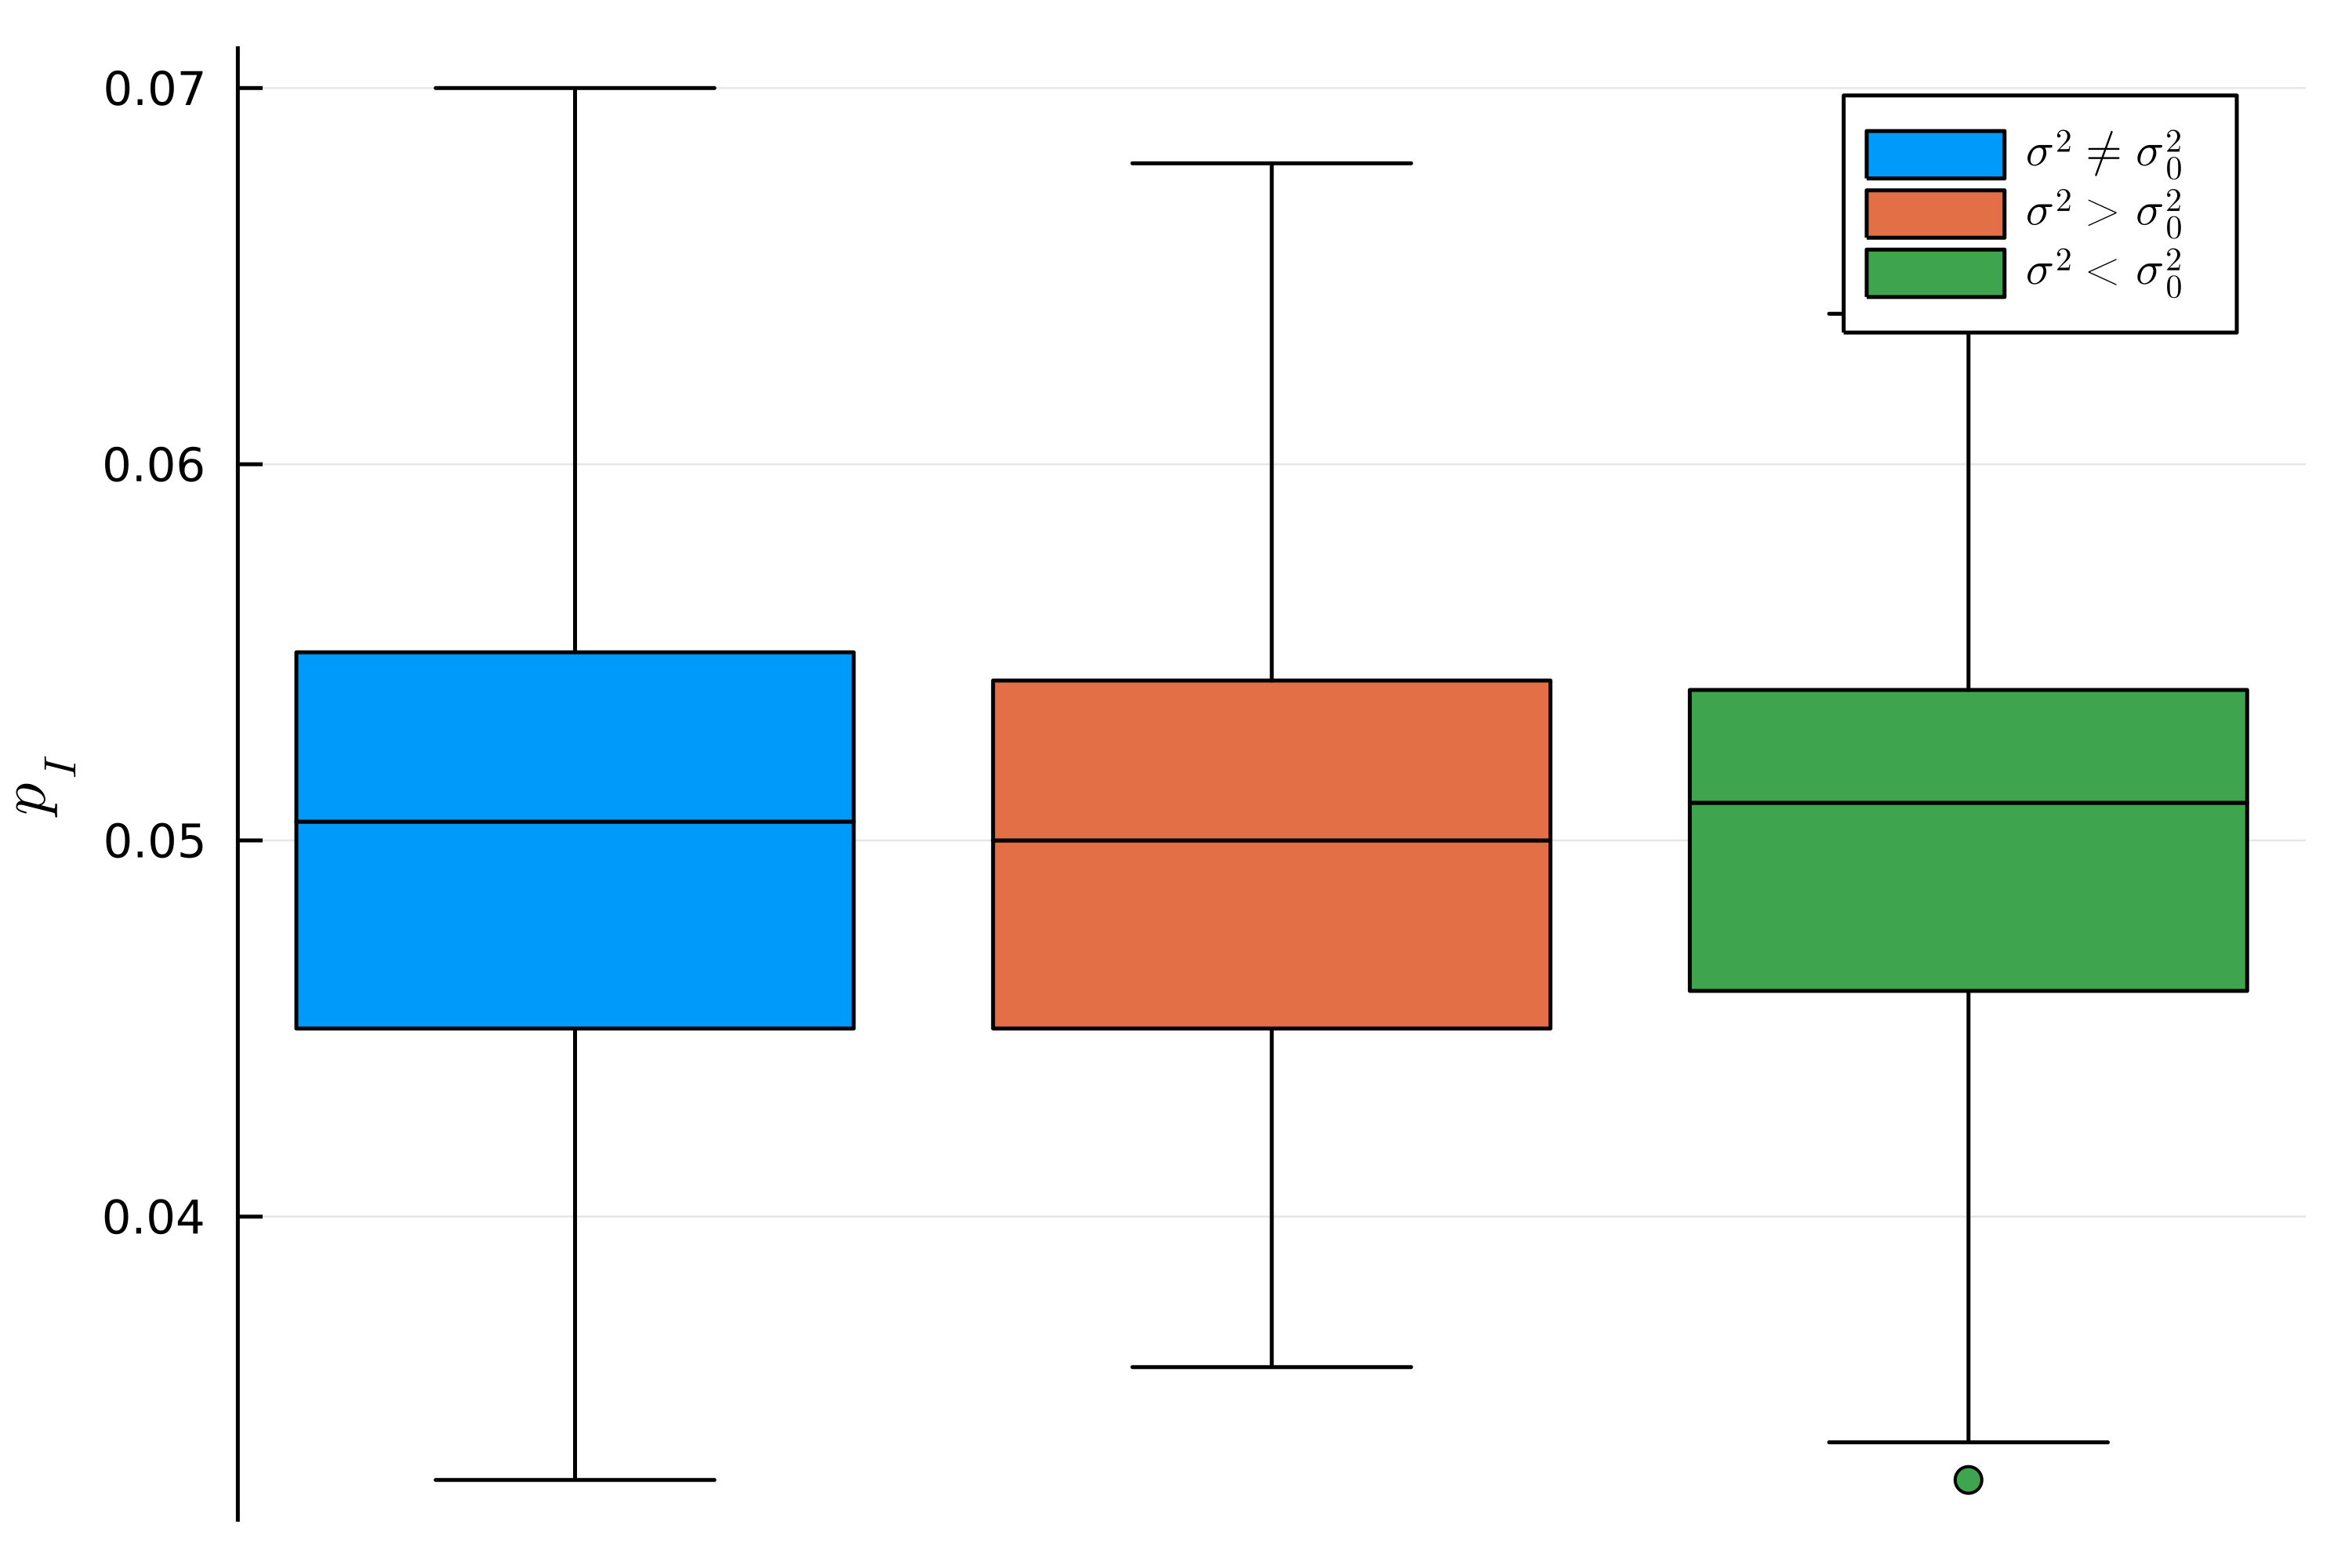
\includegraphics[scale=0.11]{images/boxplot_wariancja.png}
		\caption{Wykresy pudełkowe 100 wysymulowanych wartości prawdopodobieństwa popełnienia błędu I rodzaju dla każdej z hipotez dotyczących parametru $\sigma^2$ w drugim zadaniu.}
	\end{figure}
	
	\begin{table}[H]
		\centering
		\begin{tabular}{ |c|c|c|c| } 
			\hline
			\vphantom{ $1^{1^1}$} $\sigma^2$ \vphantom{ $1^{1^{1^1}}$} & $\sigma^2 \neq \sigma_0^2$ & $\sigma^2 > \sigma_0^2$ & $\sigma^2 < \sigma_0^2$ \\\hline
			1,47 & 0,931 & -- & 0,891 \\\hline
			1,48 & 0,951 & -- & 0,921 \\\hline
			1,49 & 0,947 & -- & 0,933 \\\hline
			1,51 & 0,922 & 0,92 & -- \\\hline
			1,52 & 0,952 & 0,925 & -- \\\hline
			1,53 & 0,927 & 0,891 & -- \\\hline
		\end{tabular}
		\caption{Wartości prawdopodobieństwa popełnienia błędu II rodzaju dla podanych w 2. zadaniu hipotez alternatywnych, wyznaczone symulacyjnie dla różnych wartości $\sigma^2$.}
	\end{table}

	\begin{table}[H]
		\centering
		\begin{tabular}{ |c|c|c|c| } 
			\hline
			\vphantom{ $1^{1^1}$} $\sigma^2$ \vphantom{ $1^{1^{1^1}}$} & $\sigma^2 \neq \sigma_0^2$ & $\sigma^2 > \sigma_0^2$ & $\sigma^2 < \sigma_0^2$ \\\hline
			1,47 & 0,069 & -- & 0,109 \\\hline
			1,48 & 0,049 & -- & 0,079 \\\hline
			1,49 & 0,053 & -- & 0,067 \\\hline
			1,51 & 0,078 & 0,08 & -- \\\hline
			1,52 & 0,049 & 0,075 & -- \\\hline
			1,53 & 0,073 & 0,109 & -- \\\hline
		\end{tabular}
		\caption{Wartości mocy testu dla podanych w 2. zadaniu hipotez alternatywnych, wyznaczone symulacyjnie dla różnych wartości $\sigma^2$.}
	\end{table}
	
	
	
	\section{Podsumowanie}
	\noindent Po przeprowadzeniu testów statystycznych dla hipotez dotyczących parametru $\mu$ w pierwszym zadaniu, wnioskujemy, że najprawdopodobniej $\mu$ jest mniejsze od 1,5. W przypadku próby z zadania drugiego testy wyraźnie wskazują, że parametr $\sigma^2$ jest większy od 1,5.\\ Następnie wyznaczyliśmy symulacyjnie prawdopodobieństwo popełnienia błędu I
	i II rodzaju dla badanych hipotez. Jak możemy zauważyć na wykresach pudełkowych, wartości prawdopodobieństwa błędu I rodzaju oscylują wokół $\alpha = 0,05$. W przypadku wyników symulacji dla błędu II rodzaju, tak jak byśmy przypuszczali, wraz ze zwiększaniem różnicy pomiędzy prawdziwym parametrem, a zakładanym w $\mathrm{H}_0$, maleje wartość prawdopodobieństwa i wzrasta moc testu.
	
	
	
	\newpage
	\begin{thebibliography}{1}
		\bibitem{zadania}
		\url{http://prac.im.pwr.edu.pl/~wyloman/statystyka_stosowana_2122/lista7.pdf}
		\bibitem{dane1}
		\url{http://prac.im.pwr.edu.pl/~wyloman/statystyka_stosowana_2122/lista7_zad1.txt}
		\bibitem{dane2}
		\url{http://prac.im.pwr.edu.pl/~wyloman/statystyka_stosowana_2122/lista7_zad2.txt}
	\end{thebibliography}


\end{document}